%%%%%%%%%%%%%%%%%%%%%%%%%%%%%%%%%%%%%%%%%%%%%%%%%%
%% Bachelor's & Master's Thesis Template        %%
%% Copyleft by Dawid Weiss & Marta Szachniuk    %%
%% Faculty of Computing and Telecommunication   %%
%% Poznan University of Technology, 2020        %%
%%%%%%%%%%%%%%%%%%%%%%%%%%%%%%%%%%%%%%%%%%%%%%%%%%


% Szkielet dla pracy licencjackiej pisanej w języku polskim.

\documentclass[polish,bachelor,a4paper,oneside]{ppfcmthesis}


\usepackage[utf8]{inputenc}
\usepackage[OT4]{fontenc}
\usepackage{hyperref}
\usepackage{float}
\usepackage{listings}
\usepackage{color}
\definecolor{lightgray}{rgb}{.9,.9,.9}
\definecolor{darkgray}{rgb}{.4,.4,.4}
\definecolor{purple}{rgb}{0.65, 0.12, 0.82}

\lstdefinelanguage{JavaScript}{
  keywords={typeof, new, true, false, catch, function, return, null, catch, switch, var, if, in, while, do, else, case, break},
  keywordstyle=\color{blue}\bfseries,
  ndkeywords={class, export, boolean, throw, implements, import, this},
  ndkeywordstyle=\color{darkgray}\bfseries,
  identifierstyle=\color{black},
  sensitive=false,
  comment=[l]{//},
  morecomment=[s]{/*}{*/},
  commentstyle=\color{purple}\ttfamily,
  stringstyle=\color{red}\ttfamily,
  morestring=[b]',
  morestring=[b]"
}

\lstset{
   language=JavaScript,
   backgroundcolor=\color{lightgray},
   extendedchars=true,
   basicstyle=\footnotesize\ttfamily,
   showstringspaces=false,
   showspaces=false,
   numbers=left,
   numberstyle=\footnotesize,
   numbersep=9pt,
   tabsize=2,
   breaklines=true,
   showtabs=false,
   captionpos=b
}


\hypersetup{
    colorlinks=false, %set true if you want colored links
    linktoc=all,     %set to all if you want both sections and subsections linked
    linkcolor=black,  %choose some color if you want links to stand out
}

%--------------------------------------
% Strona tytułowa
%--------------------------------------

% Autorzy pracy, jeśli jest ich więcej niż jeden
% wstaw między nimi separator \and
\author{%
   Mateusz Biernacki \album{140681} \and 
   Dominik Boła \album{136524} \and 
   Maciej Goral \album{132228} \and 
   Grzegorz Piątkowski \album{135868}}
\authortitle{}                                % Do not change.

\title{Aplikacja internetowa służąca do generowania planów lekcji dla szkół podstawowych oraz średnich}

% Your supervisor comes here.
\ppsupervisor{~dr~inż.~Izabela Janicka-Lipska} 

% Year of final submission (not graduation!)
\ppyear{2022}                                 


\begin{document}

% Front matter starts here
\frontmatter\pagestyle{empty}%
\maketitle\cleardoublepage%

%--------------------------------------
% Miejsce na kartę pracy dyplomowej
%--------------------------------------

\thispagestyle{empty}\vspace*{\fill}%
\vfill\cleardoublepage%

%--------------------------------------
% Spis treści
%--------------------------------------

\pagenumbering{Roman}\pagestyle{ppfcmthesis}%
\tableofcontents* 
\cleardoublepage % Zaczynamy od nieparzystej strony

%--------------------------------------
% Rozdziały
%--------------------------------------

%Najwygodniej jeśli każdy rozdział znajduje się w oddzielnym pliku
\mainmatter%

\chapter{Wstęp}
W dzisiejszych czasach ciężko znaleźć osobę która nigdy nie korzystała z internetu. Większość naszego społeczeństwa używa go na porządku dziennym. Wykorzystywany jest prawie w każdej dziedzinie życia, służyć może np. do komunikacji w czasie rzeczywistym, dokonywania szybkich płatności, zakupów internetowych, nauki czy też pracy. Przykłady można wymieniać bez końca, jednak trzeba zwrócić szczególną uwagę na narzędzia, dzięki którym możemy korzystać z sieci w tak szerokim zakresie. Jednym z najpopularniejszych wykorzystywanych oraz dynamicznie rozwijanych rozwiązań są aplikacje webowe. Jedną z ich głównych zalet jest możliwość korzystania z nich niezależnie od używanego urządzenia, o ile ma ono dostęp do internetu oraz posiada przeglądarkę internetową. W przeciwieństwie do aplikacji desktopowych, wszelkie aktualizację są dokonywane przez administratora, co w kontekście rozwoju oprogramowania jest bardzo wygodne zarówno dla programisty jak i użytkownika. Są to jedne z wielu zalet, które z pewnością przyczyniły się do szybkiego rozwoju aplikacji internetowych oraz związanych z nimi technologii.

Tematem podjętym w pracy jest aplikacja służąca do generowania planów zajęć. Zaprojektowanie tego typu rozwiązania, daje możliwość nauki rozmaitych technologii informatycznych, powszechnie wykorzystywanych w praktyce. Główną motywacją do podjęcia takiego tematu stanowią wady obecnie stosowanego przez większość szkół manualnego tworzenia planów zajęć. Ręczne tworzenie planu jest czasochłonne i wymaga dużego nakładu pracy. Dla osób odpowiedzialnych za ich przygotowanie (dalej zwanych planistami) jest to zadanie monotonne, a także przytłaczające. Planiści, nawet ci z dużym doświadczeniem, nie są zdolni do utworzenia planu, który optymalnie wykorzystywałby godziny uczniów, nauczycieli, a także dostępność sali lekcyjnych. Skutkuje to znaczną liczbą niewykorzystanego czasu w środku dnia lekcyjnego.

Celem pracy jest zaprojektowanie aplikacji, dzięki której po podaniu niezbędnych danych, możliwe byłoby automatyczne wygenerowanie planu zajęć dla szkoły. Aplikacja ma umożliwić planiście dodawanie danych o przedmiotach, nauczycielach, salach i klasach. Na podstawie podanych danych planista ma mieć możliwość generacji rozkładu zajęć dla wszystkich klas w szkole. Aplikacja ma być przeznaczona dla szkół podstawowych oraz średnich. Ograniczenie to wynika z założenia niepodzielności klasy. W przypadku uczelni wyższych niejednolity podział na grupy znacząco zwiększa poziom skomplikowania rozwiązywanego problemu. 

Projekt można podzielić na cztery główe części: konfigurację infrastruktury informatycznej, implementację back-end, implementację front-end oraz implementację algorytmu.

Praca ma następującą strukturę. Rozdział drugi poświecony jest podstawom teoretycznym. Rozdział trzeci zawiera analizę problemu i dostępnych rozwiązań. Rozdział czwarty to opis metodyki pracy oraz infrakstruktury informatycznej. Rozdział piąty omawia część fronendową aplikacji. Rozdział szósty charakteryzuje backend aplikacji. Rozdział siódmy wyjaśnia działanie algorytmu generacji planu. Rozdział ósmy jest instrukcją użytkowania. Rozdział dziewiąty stanowią wnioski. 

Implementacja aplikacji została wykonana przez cztery osoby.
Mateusz Biernacki wykonał ...
Dominik Boła wykonał ...
Maciej Goral wykonał ...
Grzegorz Piątkowski wykonał ...

% Co to jest NP - https://dbpedia.org/page/NP_(complexity)
% Co to jest problem NP-Trudny - https://www.baeldung.com/cs/p-np-np-complete-np-hard
% Ułozenie planu zajęć jako problem np-trudny - https://www.sciencedirect.com/science/article/pii/S1110016816000703#b0015


\chapter{Podstawy teoretyczne}
Wygenerowanie najlepszego możliwego planu zajęć dla dużej szkoły jest problemem NP-zupełnym. Liczba wszystkich możliwych do ułożenia poprawnych planów zajęć rośnie wykładniczo, wraz z wielkością szkoły, dla której plan jest tworzony. Nie jest możliwa, w rozsądnym przedziale czasowym, iteracja przez wszystkie rozwiązania i wybranie najlepszego z nich. Należy skorzystać z rozwiązania, które dostarczy rozwiązanie dobre, jak najbardziej zbliżone do optymalnego. Uzyskanie takiego wyniku umożliwia wykorzystanie podejścia ewolucyjnego.

Rozdział teoretyczny --- przegląd literatury naświetlający stan wiedzy na dany temat. 

Przegląd literatury naświetlający stan wiedzy na dany temat obejmuje rozdziały pisane na podstawie
literatury, której wykaz zamieszczany jest w części pracy pt.~\emph{Literatura} (lub inaczej \emph{Bibliografia},
\emph{Piśmiennictwo}). W tekście pracy muszą wystąpić odwołania do wszystkich pozycji zamieszczonych w
wykazie literatury. \textbf{Nie należy odnośników do literatury umieszczać w stopce strony.} Student jest
bezwzględnie zobowiązany do wskazywania źródeł pochodzenia informacji przedstawianych w pracy,
dotyczy to również rysunków, tabel, fragmentów kodu źródłowego programów itd. Należy także podać
adresy stron internetowych w przypadku źródeł pochodzących z Internetu.



\chapter{Analiza i porównanie możliwych rozwiązań}
\section{Analiza problemu}
Podstawowym problemem w automatycznym tworzeniu planu zajęć jest dobór warunków wykorzystywanym przy generacji. Warunki te można podzielić na niezbędne do utworzenia poprawnego planu oraz warunki dodatkowe, których spełnienie zwiększa użyteczność planu z punktu widzenia planisty. 

Wśród warunków niezbędnych należy wyróżnić warunek braku konfliktów. Konflikt ma miejsce, gdy występuje jedna z następujących sytuacji:
\begin{itemize}
    \item w jednej godzinie lekcyjnej, jednej klasie została przyporządkowana więcej niż jeden przedmiot,
    \item w jednej godzinie lekcyjnej, jednemu nauczycielowi została przyporządkowana więcej niż jedna klasa,
    \item w jednej godzinie lekcyjnej jednej sali została przyporządkowana więcej niż jedna klasa.
\end{itemize}
W przypadku szkół podstawowych oraz średnich do warunków niezbędnych należy również zaliczyć brak niewykorzystanych godzin w środku dnia lekcyjnego dla uczniów. Dodatkowo niektóre zajęcia, takie jak wychowanie fizyczne, mogą być przeprowadzone tylko w specjalnie przeznaczonych do tego salach.

Warunki dodatkowe mogą różnić się w zależności od czynników, które należy wziąć pod uwagę przy pod uwagę przy generacji plany wynikające ze specyfikacji szkoły oraz wymagań personelu dydaktycznego. Do tych czynników można zaliczyć:
\begin{itemize}
    \item ograniczenia dostępności nauczycieli, wynikające z pracy w innych placówkach oświatowych lub innych powodów,
    \item ograniczenia wynikające z odległości między salami,
    \item obecność zajęć nieobowiązkowych, które muszą w danym dniu lekcyjnym być skrajnie pierwsze lub ostatnie,
    \item  minimalizację niewykorzystanych godzin w środku dnia lekcyjnego dla uczniów,
    \item konieczność grupowania zajęć w przypadku kilku godzin lekcyjnych tego samego przedmiotu jednego dnia -- w takim przypadku zajęcia te powinny następować bezpośrednio po sobie oraz w tej samej sali,
    \item możliwie jak najbardziej równomierne rozłożenie przedmiotów trakcie tygodnia lekcyjnego.
\end{itemize}
\section{Aktualnie dostępne rozwiązania}
\subsection{aSc TimeTables}
aSc TimeTables~\cite{asc} to aplikacja desktopowa wspomagająca przygotowywanie planów zajęć. Narzędzie umożliwia generowanie planów na podstawie zdefiniowanych wymagań, wprowadzenie do nich ręcznych poprawek oraz wyszukiwanie konfliktów we wprowadzonych zmianach. aSc TimeTables jest najbardziej rozbudowanym rozwiązaniem tego typu dostępnym na rynku, pozwalającym na tworzenie planów zajęć dla szkół i uczelni. Do dodatkowych funkcji programu należy możliwość importu danych z pliku, zdolność mapowania szkoły oraz udostępnienia planów uczniom i nauczycielom za pomocą aplikacji mobilnej. Z wszechstronnością i bogactwem funkcji wiąże się wysoki poziom umiejętności potrzebny do poprawnego wykorzystania aplikacji. Do pozostałych wad programu należy brak regularnych aktualizacji, podatność na błędy w generacji planu, wysoka cena oraz dostępność ograniczona do systemu Windows.
\subsection{Prime Timetable}
Prime Timetables~\cite{prime} to aplikacja internetowa przeznaczona dla organizacji edukacyjnych umożliwiająca zarówno ręczne jak i automatyczne układanie planów lekcji. Prime Timetables pozwala na wspólne tworzenie planów przez kilku użytkowników oraz udostępnianie gotowych planów dla uczniów i nauczycieli posiadających konta w serwisie. Aplikacja posiada rozbudowany zestaw narzędzi umożliwiających określanie ograniczeń związanych z automatyczną generacją planu. Główną wadą rozwiązania jest wysoka opłata miesięczna, której wysokość dodatkowo zależy od liczby nauczycieli w szkole. 
\subsection{SuperSaas}
SuperSaas~\cite{saas} to program do zarządzania szkołami i innymi instytucjami, którego głównym atutem jest wbudowany system rezerwacji. Przy pomocy konta WordPress użytkownicy aplikacji mogą umawiać terminy wizyt, a także dokonywać za nie płatności. SuperSaas cechuje niska cena oraz dostępność z poziomu przeglądarki. Duża część funkcjonalności aplikacji nie jest przeznaczona dla szkół. Pomimo możliwości wspomagania ręcznego układania planów zajęć, program nie pozwala na automatyczną ich generację, ani nawet wykrywanie konfliktów. 
\section{Możliwe podejścia}
Możliwe rozwiązania można podzielić w zależności od kilku aspektów. Pierwszym z nich jest wybór rodzaju aplikacji -- desktopowej, mobilnej lub internetowej. Ze względu na fakt, że korzystanie z aplikacji wymagać ma wprowadzania dużej ilości danych można założyć, że z punktu widzenia użytkownika najwygodniejsze będzie użycie w tym celu fizycznej klawiatury. Powoduje to odrzucenie wyboru aplikacji mobilnej. Zaletami  wyboru aplikacji desktopowej jest możliwość korzystania z niej bez dostępu do internetu oraz bezpieczeństwo związane z lokalnym przechowywaniem danych. Pomimo tych korzyści rozwiązanie to nie oferuje zalet związanych z wyborem aplikacji internetowej -- dostępu z dowolnego urządzenia wyposażonego w kompatybilną przeglądarkę, braku wymagań systemowych związanych z obliczeniami i przechowywaniem danych oraz braku konieczności aktualizowania aplikacji przez użytkownika.
\section{Wymagania funkcjonalne i niefunkcjonalne}
\section{Przypadki użycia}

\chapter{Metodyka pracy oraz przygotowanie infrastruktury informatycznej}

\section{Wstęp}
Projekt powstawał w metodyce DevOps. Takie podejście pozwoliło na szybsze dostarczenie finalnego produktu. Wysoki poziom kooperacji wynikający z metodki DevOps pozwolił na zmniejszenie kosztów dostarczenia produktu oraz znaczne zwiększenie jego spójności. Potrzebna jest jednak mocno rozwinięta infrastruktura informatyczna służąca podtrzymaniu DevOps lifecycle.

\section{Pojęcia}
	\subsection{DevOps}
	DevOps~\cite{devops} to zestaw praktyk, narzędzi i filozofii kulturowej, które automatyzują i integrują procesy pomiędzy zespołami programistów oraz IT. Kładzie nacisk na wzmocnienie pozycji zespołu, komunikację i współpracę między zespołami oraz automatyzację technologii.
	Ruch DevOps rozpoczął się około 2007 roku, kiedy społeczności programistów i operatorów IT wyraziły zaniepokojenie tradycyjnym modelem rozwoju oprogramowania, w którym programiści piszący kod pracowali oddzielnie od operatorów, którzy wdrażali i wspierali kod. Termin DevOps, będący połączeniem słów \textit{development} i \textit{operations}, odzwierciedla proces integracji tych dyscyplin w jeden, ciągły proces (zob.~rysunek~\ref{rys:devops_lifecycle}).
\begin{figure}[H]
\centering\includegraphics[width=10cm]{figures/devops_lifecycle}
\caption{Schemat DevOps lifecycle~\cite{devops_lifecycle}}\label{rys:devops_lifecycle}
\end{figure}

	\subsection{Continous Integration and Continous Deployment}
	\textit{Continous Integration and Continous Deployment} (CI/CD)~\cite{ci} to metoda częstego dostarczania aplikacji do klientów poprzez wprowadzenie automatyzacji do etapów tworzenia aplikacji. Główne pojęcia przypisane do CI/CD to ciągła integracja, ciągłe dostarczanie i ciągłe wdrażanie. CI/CD jest rozwiązaniem problemów, jakie integracja nowego kodu może powodować dla zespołów programistycznych i operacyjnych.
	W szczególności, CI/CD wprowadza ciągłą automatyzację i ciągłe monitorowanie w całym cyklu życia aplikacji, od fazy integracji i testowania po dostarczanie i wdrażanie. Łącznie, te połączone praktyki są często określane jako CI/CD i są wspierane przez zespoły programistów i operatorów pracujących razem z podejściem DevOps lub SRE (\textit{site reliability engineering}).
	
	\subsection{Kontrola wersji}
	Kontrola wersji~\cite{version_control}, znana również jako kontrola źródła, jest praktyką śledzenia i zarządzania zmianami w kodzie oprogramowania. Systemy kontroli wersji to narzędzia programowe, które pomagają zespołom programistów zarządzać zmianami w kodzie źródłowym w czasie.


\section{Narzędzia i technologie}
	\subsection{Amazon Web Services}
	\textit{Amazon Web Services} (AWS)~\cite{aws} jest spółką zależną firmy Amazon, dostarczającą platformy chmury obliczeniowej na żądanie oraz interfejsy API osobom prywatnym, firmom i rządom na zasadzie \textit{pay-as-you-go}. Te usługi internetowe w chmurze obliczeniowej zapewniają różnorodne podstawowe abstrakcyjne elementy infrastruktury technicznej oraz narzędzia i bloki do obliczeń rozproszonych. Jedną z tych usług jest \textit{Amazon Elastic Compute Cloud} (EC2), która pozwala użytkownikom mieć do dyspozycji wirtualny klaster komputerów, dostępny przez cały czas, przez Internet. Wirtualne komputery AWS emulują większość atrybutów prawdziwego komputera, w tym sprzętowe jednostki centralne (CPU) i procesory graficzne (GPU) do przetwarzania danych, pamięć lokalną/RAM, pamięć masową HDD/SSD, wybór systemów operacyjnych, sieci oraz wstępnie załadowane oprogramowanie użytkowe, takie jak serwery internetowe, bazy danych i zarządzanie relacjami z klientami (CRM).
	
	\subsection{Git}
	Git~\cite{git} to darmowe narzędzie open-source służące do kontroli wersji, zaprojektowane do obsługi wszystkiego, od małych do bardzo dużych projektów z dużą prędkością i wydajnością.	
	
	\subsection{GitHub}
	GitHub~\cite{github} jest dostawcą hostingu internetowego dla rozwoju oprogramowania i kontroli wersji przy użyciu Git. Oferuje on funkcje rozproszonej kontroli wersji i zarządzania kodem źródłowym (SCM) Git, a także własne funkcje.
	
	\subsection{Docker}
	Docker~\cite{docker} to platforma konteneryzacji typu open source. Umożliwia ona programistom pakowanie aplikacji w kontenery -- ustandaryzowane komponenty wykonywalne łączące kod źródłowy aplikacji z bibliotekami systemu operacyjnego (OS) i zależnościami wymaganymi do uruchomienia tego kodu w dowolnym środowisku. Kontenery upraszczają dostarczanie aplikacji rozproszonych i stają się coraz bardziej popularne w miarę jak organizacje przechodzą na rozwój cloud-native i hybrydowe środowiska wielochmurowe.
	
	\subsection{CircleCI}
	CircleCI~\cite{circleci} jest platformą obsługującą \textit{Continous Integration and Continous Delivery} (CI/CD), która pomaga zespołom programistycznym szybko i pewnie wypuszczać kod poprzez możliwość tworzenia \textit{pipeline} (brak odpowiednika w języku polskim) automatyzujących proces budowania, testowania i wdrażania. Pozwala to zespołom szybko się rozwijać, łatwo skalować i budować spójne produkty (zob.~rysunek~\ref{rys:circleci_diagram}).
	\begin{itemize}
	\item \textit{Pipeline} jest jednostką pracy najwyższego poziomu, obejmującą cały plik ,,.circleci/config.yml'' projektu. \textit{Pipeline} zawiera przepływy pracy (\textit{workflow}), które koordynują zadania. Mają one ustalony, liniowy cykl życia i są powiązane z konkretnym aktorem. \textit{Pipeline} uruchamia się po wprowadzeniu zmiany do projektu, który zawiera plik konfiguracyjny CircleCI, a także może być zaplanowany, uruchamiany ręcznie za pomocą aplikacji CircleCI lub interfejsu API.
	\end{itemize}
\begin{figure}[H]
\centering\includegraphics[width=\textwidth]{figures/circleci_schema}
\caption{Diagram przedstawiający działanie CircleCI~\cite{circleci_schema}}\label{rys:circleci_diagram}
\end{figure}

	\subsection{Secure Shell}
	\textit{Secure Shell} (SSH)~\cite{ssh} to protokół zdalnej administracji, który pozwala użytkownikom kontrolować i modyfikować zdalne serwery przez Internet. Usługa ta została stworzona jako bezpieczny zamiennik dla nieszyfrowanego protokołu Telnet i wykorzystuje techniki kryptograficzne, aby zapewnić szyfrowaną komunikację ze zdalnym serwerem. Zapewnia mechanizm uwierzytelniania zdalnego użytkownika, przesyłania danych wejściowych od klienta do hosta i przekazywania danych wyjściowych z powrotem do klienta.
	
	\subsection{tmux}
	tmux~\cite{tmux} jest multiplekserem terminali. Umożliwia tworzenie, dostęp i sterowanie wieloma terminalami z jednego ekranu. tmux może zostać odłączony od ekranu i kontynuować pracę w tle, a następnie ponownie dołączony.
	
	\subsection{shell}
	\textit{Shell}~\cite{shell} to termin UNIX dla interaktywnego interfejsu pośredniczącego między użytkownikiem a systemem operacyjnym. \textit{Shell} jest warstwą programowania, która rozumie i wykonuje polecenia wprowadzane przez użytkownika. W niektórych systemach, powłoka nazywana jest interpreterem poleceń. \textit{Shell} zwykle implikuje interfejs ze składnią poleceń.
	
	\subsection{Black}
	Black~\cite{black} jest formaterem kodu w języku Python. Wykorzystanie gotowego rozwiązania oraz zastosowanie go dla wszystkich plików  ,,.py'' standaryzuje kod co znacznie ułatwia pracę nad większym projektem.
	
	\subsection{Pylint}
	Pylint~\cite{pylint} jest narzędziem do statycznej analizy kodu w języku Python. Pylint szuka błędów programistycznych, pomaga egzekwować standardy kodowania i oferuje proste sugestie refaktoryzacji.

\section{Przygotowanie infrastruktury informatycznej}
	\subsection{Przygotowanie strony serwerowej przy pomocy platformy AWS}
	Do przygotowania strony serwerowej aplikacji wykorzystano jedną z usług platformy \textit{Amazon Web Services} jaką jest \textit{Amazon Elastic Compute Cloud} (EC2). Do przygotowania serwera strony frontendowej oraz backendowej przygotowano dwie niezależne instancje usługi EC2. Obie z przygotowanych instancji są typu \textit{t2.micro} zawierającego się w ramach pakietu \textit{AWS Free Tier}. Dzięki wyborowi tego typu instancji udało się zachować zerowy wkład pieniężny na potrzeby pracy inżynierskiej. Zasoby możliwe do wykorzystania w ramach typu \textit{t2.micro} nie są wystarczające na przypadek skomercjalizowania projektu jednak w zupełności wystarczają na potrzeby przygotowania projektu w ramach pracy inżynierskiej.
System operacyjny wykorzystany na obu instancjach EC2 to \textit{Linux Ubuntu 20.04.3 LTS} w wersji serwerowej. Zastosowanie takiej wersji systemu zmniejsza zapotrzebowanie systemu na zasoby obliczeniowe przez ograniczenie procesów systemowych (np. brak GUI) dzięki czemu większa ilość zasobów może zostać udostępniona na potrzeby zadań serwerowych. W celu zwiększenia bezpieczeństwa komunikacji, reguły połączeń przychodzących (\textit{Inbound Rules}) oraz reguły połączeń wychodzących (\textit{Outbound Rules}) zostały skonfiguorwane tak, aby jak najbardziej uszczegółowić typy możliwych połączeń z instancjami.
	
	\subsection{Przygotowanie CI/CD Pipeline przy pomocy platformy CircleCI}
	Do przygotowania \textit{CI/CD pipeline} wykorzystano platformę CircleCI. Cały proces przygotowano w taki sposób, aby \textit{pipeline} uruchamiany został w momencie wprowadzenia zmian w repozytorium. Zadanie (\textit{job}) budowania (\textit{build}) i testowania (\textit{test}) uruchamiane jest dla każdych zmian wprowadzonych w zdalnym repozytorium. Zadanie wdrażania (\textit{deployment}) uruchamiane jest tylko i wyłącznie, jeśli zmiany zostały wprowadzone w ramach gałęzi Git (\textit{branch}) \textit{main} oraz jeśli zadanie budowania i testowania zakończyło się bez błędów (zob.~rysunek~\ref{rys:passed_ppl} oraz ~rysunek~\ref{rys:error_ppl}).

	
\begin{figure}[H]
\centering\includegraphics[width=\textwidth]{figures/ppl_flow}
\caption{Pipeline uruchomiony dla zmian wprowadzonych w gałęzi Git \textit{main}.}\label{rys:passed_ppl}
\end{figure}

\begin{figure}[H]
\centering\includegraphics[width=\textwidth]{figures/ppl_flow_fail}
\caption{Pipeline, w którym wystąpiły błędy. Uruchomiony dla zmian wprowadzonych w gałęzi Git innej niż \textit{main}.}\label{rys:error_ppl}
\end{figure}

	Każdy przepływ pracy składa się z zadań, na które składają się jeszcze mniejsze kroki, podczas których wywoływane mogą być polecenia interfejsu \textit{shell}, wykonywane w kontenerach Docker stworzonych na potrzeby wykonania danego zadania. Platforma CircleCI umożliwia tworzenie własnych obrazów Docker jak i zarówno dostarcza szereg gotowych rozwiązań przygotowanych w celu ułatwienia i przyśpieszenia tworzenia \textit{pipeline} na potrzeby małych projektów. Na potrzeby projektu inżynierskiego utworzono przepływ pracy \textit{build\_test\_deploy} składający się z 4 zadań \textit{build\_and\_test\_back, build\_and\_test\_front, deploy\_frontend} oraz \textit{deploy\_backend} (zob.~listing~\ref{lst:workflow}).
	
\newpage
\begin{itemize}
	\item \textit{build\_and\_test\_back} -- podczas tego kroku budowany jest kontener Docker na bazie obrazu z przygotowanym Pythonem w wersji 3.9. Na początku tego zadania w obrębie kontenera wykonywane jest przełączenie (\textit{checkout}) na gałąź Git, której zmiany wywołały start \textit{pipeline}. Następnie wykonywany jest krok instalujący wymagania projektowe (\textit{requirements}) z pliku ,,requirements.txt''. Kolejnym krokiem jest sformatowanie plików ,,.py'' przy pomocy gotowego rozwiązania jakim jest narzędzie Black. Następny krok to sprawdzenie kodu przy pomocy Pylint. Wykorzystanie tego narzędzia zwiększa jakość publikowanego kodu oraz go standaryzuje w przypadku rozwijania oprogramowania przez wiele osób. Dwa ostatnie kroki odpowiedzialne są za uruchomienie testów jednostkowych backendu oraz algorytmu (zob.~listing~\ref{lst:test_back} oraz ~rysunek~\ref{rys:test_back}).
	\item \textit{build\_and\_test\_front} -- w tym zadaniu na początku budowany jest kontener Docker na bazie obrazu z przygotowanym Node.js w wersji 17.2.0. Następnie wykonywane jest przełączenie do gałęzi Git, której zmiany wywołały start \textit{pipeline}.  Kolejne dwa kroki odpowiedzialne są za przygotowanie środowiska tj. zaktualizowanie wersji Node.js do \textit{latest} oraz zainstalowanie dependencji projektu. W tak przygotowanym środowisku ostatnim krokiem jest uruchomienie testów jednostkowych z przygotowanego pliku (zob.~listing~\ref{lst:test_front} oraz ~rysunek~\ref{rys:test_front}).
	\item \textit{deploy\_frontend} -- w tym zadaniu głównym narzędziem jest aws-cli (\textit{AWS command line interface}). Pozwala on na obsługę instancji EC2 z poziomu interfejsu \textit{shell}. Pierwszym krokiem zadania jest przełączenie do gałęzi Git, której zmiany wywołały wystartowanie \textit{pipeline}. W nastepnym kroku ustawiany jest \textit{access\_key\_id} oraz \textit{secret\_access\_key} potrzebny do połączenia SSH. Dzięki wykorzystaniu zmiennych środowiskowych platformy CircleCI wartości te pozostają ukryte dla osób nie mających dostępu do projektu z poziomu platformy. Ostatnim, jednak bardzo rozbudowanym krokiem, jest połączenie z użyciem protokołu SSH i wykonanie operacji wdrożenia z poziomu instancji serwera. Po podłączeniu się do maszyny zdalnej wykonywane są takie czynności jak pobranie (\textit{pull}) najnowszych zmian ze zdalnego repozytorium, reinstalacja dependencji oraz restart serwera frontendowego. Po stronie serwera wykorzystywane jest narzędzie tmux. Dzięki otwarciu sesji w tle, możliwe jest wykonywanie innych czynności z równolegle działającym serwerem oraz utrzymanie sesji serwera po zakończeniu sesji \textit{SSH} (zob.~listing~\ref{lst:deploy_front} oraz ~rysunek~\ref{rys:deploy_front}).
	\item \textit{deploy\_backend} -- podobnie jak w zadaniu \textit{deploy\_frontend} głównym narzędziem jest aws-cli. Pierwszym krokiem zadania jest przełączenie do gałęzi Git, której zmiany wywołały wystartowanie \textit{pipeline}. W następnym kroku ustawiany jest \textit{access\_key\_id} oraz \textit{secret\_access\_key} potrzebny do połączenia SSH. Dzięki wykorzystaniu zmiennych środowiskowych platformy CircleCI wartości te pozostają ukryte dla osób nie mających dostępu do projektu z poziomu platformy. Ostatnim krokiem jest połączenie z użyciem protokołu SSH i wykonanie operacji wdrożenia z poziomu instancji serwera. Po rozpoczęciu sesji zdalnej z instancją serwera, wykonywane są takie czynności jak pobranie najnowszych zmian ze zdalnego repozytorium, reinstalacja wymagań projektowych z pliku ,,requirements.txt'' oraz restart serwera backendowego. Po stronie serwera wykorzystywane jest narzędzie tmux (zob.~listing~\ref{lst:deploy_back} oraz ~rysunek~\ref{rys:deploy_back}).
\end{itemize}
	
\newpage
	
\begin{lstlisting}[caption=Część skryptu config.yml odpowiedzialna za określenie przepływów pracy,label={lst:workflow}]
workflows:
  build_test_deploy:
    jobs:
      - build_and_test_back
      - build_and_test_front
      - deploy_frontend:
          requires:
            - build_and_test_back
            - build_and_test_front
          filters:
            branches:
              only:
                - main
      - deploy_backend:
          requires:
            - build_and_test_back
            - build_and_test_front
          filters:
            branches:
              only:
                - main
\end{lstlisting} 


	
\begin{lstlisting}[caption=Część skryptu config.yml odpowiadająca za wykonanie zadania \textit{build\_and\_test\_back},label={lst:test_back}]
build_and_test_back:
    docker:
      - image: cimg/python:3.9
    steps:
      - checkout
      - run:
          name: Install requirements
          command:
            sudo apt-get update;
            pip install --upgrade pip && pip install -r requirements.txt && pip install pylint
      - run:
          name: Format .py files
          command:
            pip install black && black $(git ls-files '*.py')
      - run:
          name: pylint
          command:
            pylint $(git ls-files '*.py')
      - run:
          name: unit_test_django
          command:
            cd Backend && python manage.py test backend_api
      - run:
          name: unit_test_algorithm
          command:
            cd Algorithm && pytest
\end{lstlisting} 
\begin{figure}[H]
\centering\includegraphics[width=14cm]{figures/circleci_test_back}
\caption{Przykładowy przebieg zadania \textit{build\_and\_text\_back}. Uruchomiony dla zmian wprowadzonych w gałęzi Git \textit{main}.}\label{rys:test_back}
\end{figure} 


\begin{lstlisting}[caption=Część skryptu config.yml odpowiadająca za wykonanie zadania \textit{build\_and\_test\_front},label={lst:test_front}]
build_and_test_front:
    docker:
      - image: cimg/node:17.2.0
    steps:
      - checkout
      - run:  
          name: Update node.js
          command:
            npm install node.js@latest
      - run:
          name: Install dependencies
          command:
            npm install ./Frontend
      - run:
          name: unit_tests
          command:
            cd Frontend &&
            npm run test:unit
\end{lstlisting}
\newpage
\begin{figure}[H]
\centering\includegraphics[width=14cm]{figures/circleci_test_front}
\caption{Przykładowy przebieg zadania \textit{build\_and\_text\_front}. Uruchomiony dla zmian wprowadzonych w gałęzi Git \textit{main}.}\label{rys:test_front}
\end{figure}
	
\begin{lstlisting}[caption=Część skryptu config.yml odpowiadająca za wykonanie zadania \textit{deploy\_frontend},label={lst:deploy_front}]
deploy_frontend:
    executor: aws-cli/default
    steps:
      - checkout
      - aws-cli/setup:
          aws-access-key-id: AWS_ACCESS_KEY_ID_FRONT
          aws-secret-access-key: AWS_SECRET_ACCESS_KEY_FRONT
      - run:
          name: deploy_frontend
          command: |
            sudo apt-get update
            # SSH to the server to deploy and Perform steps to deploy
            ssh -o StrictHostKeyChecking=no $EC2_USERNAME@$EC2_PUBLIC_DNS_FRONT 'cd GroupProject; 
            git pull --rebase;
            cd Frontend;
            npm install;
            tmux kill-session -t FRONTEND_SERVER
            sleep 5;
            tmux new-session -d -s "FRONTEND_SERVER";
            tmux send-keys -t FRONTEND_SERVER "npm run serve" C-m;
            exit'
\end{lstlisting}
\newpage
\begin{figure}[H]
\centering\includegraphics[width=14cm]{figures/circleci_deploy_front}
\caption{Przykładowy przebieg zadania \textit{deploy\_frontend}. Uruchomiony dla zmian wprowadzonych w gałęzi Git \textit{main}.}\label{rys:deploy_front}
\end{figure}


\begin{lstlisting}[caption=Część skryptu config.yml odpowiadająca za wykonanie zadania \textit{deploy\_backend},label={lst:deploy_back}]
deploy_backend:
    executor: aws-cli/default
    steps:
      - checkout
      - aws-cli/setup:
          aws-access-key-id: AWS_ACCESS_KEY_ID_BACK
          aws-secret-access-key: AWS_SECRET_ACCESS_KEY_BACK
      - run:
          name: deploy_back
          command: |
            sudo apt-get update
            # SSH to the server to deploy and Perform steps to deploy
            ssh -o StrictHostKeyChecking=no $EC2_USERNAME@$EC2_PUBLIC_DNS_BACK 'cd GroupProject; 
            git pull --rebase;
            python -m pip install -r requirements.txt;
            cd Backend;
            tmux kill-session -t BACKEND_SERVER
            tmux new-session -d -s "BACKEND_SERVER";
            tmux send-keys -t BACKEND_SERVER "python3 manage.py runserver 0.0.0.0:8000" C-m;
            exit'
\end{lstlisting}
\newpage
\begin{figure}[H]
\centering\includegraphics[width=\textwidth]{figures/circleci_deploy_back}
\caption{Przykładowy przebieg zadania \textit{deploy\_backend}. Uruchomiony dla zmian wprowadzonych w gałęzi Git \textit{main}.}\label{rys:deploy_back}
\end{figure}


	\subsection{Zastosowanie DevOps lifecycle od strony GitHub}
	W celu zwiększenia jakości dostarczanych rozwiązań zastosowano następujący przebieg wdrażania. Członek zespołu, chcąc wprowadzić nową funkcjonalność lub rozwinąć już istniejącą, zaciąga najnowszą wersję projektu ze zdalnego repozytorium. Gdy lokalne repozytorium jest zaktualizowane, deweloper tworzy nową gałąź Git, w której będzie wprowadzał zmiany. W momencie gdy autor chce podzielić się swoją pracą z innymi członkami zespołu, publikuje (\textit{push}) swoje zmiany do zdalnego repozytorium oraz tworzy \textit{Pull Request} (PR). W takim PR można prześledzić wszystkie zmiany jakie zostały po kolei wprowadzone przez autora. Każda wprowadzona zmiana pojawiająca się w zdalnym repozytorium wywołuje uruchomienie \textit{pipeline} na platformie CircleCI. Wynik działania zadań z uruchomionego przepływu pracy \textit{pipeline} również można sprawdzić z poziomu PR. W przypadku gdy zmiany wprowadzone w ramach PR przechodzą wszystkie testy oraz nie wywołują żadnych konfliktów, autor prosi o sprawdzenie i zatwierdzenie zmian przez innego członka zespołu. Gdy współpracownik zatwierdzi zmiany, gałąź Git stworzona przez autora na potrzeby zmian może zostać scalona (\textit{merge}) z gałęzią Git \textit{main}. Po wprowadzeniu zmian do gałęxi Git \textit{main} następuje ostatni etap tj. uruchomienie \textit{pipeline} z poziomu tej gałęzi a co za tym idzie, ponowne zbudowanie i przetestowanie aplikacji oraz ostatecznie wdrożenie (zob.~rysunek~\ref{rys:github}).
\begin{figure}[H]
\centering\includegraphics[width=\textwidth]{figures/github_pr}
\caption{Przykładowy przebieg wdrażania zmian przy pomocy \textit{Pull Request}}\label{rys:github}
\end{figure}
	
	 

\chapter{Projekt i implementacja aplikacji internetowej w technologii Vue.js}
\section{Narzędzia i techonologie}
\subsection{Node.js}
Node.js~\cite{node} jest środowiskiem uruchomieniowym umożliwiającym używanie języka JavaScript poza przeglądarką. Środowisko to charakteryzuje asynchroniczność oraz sterowanie zdarzeniami. Asynchroniczność umożliwia wykonywanie wielu czynności w tym samym czasie bez względu na jednowątkowość wynikającą z ograniczenia języka JavaScript. Sterowanie zdarzeniami jest rozwiązaniem typowym dla interfejsów graficznych. Zapewnia ono elastyczność oraz możliwość tworzenia bardziej interaktywnych elementów GUI. Ponadto Node.js udostępnia menenadżera pakietów środowiska Node (NPM -- Node Package Manager) dającego możliwość zarządzania zainstalowanymi funkcjonalnościami w prosty i przejrzysty sposób.
\subsection{Vue.js}
Vue.js~\cite{vue} to platforma programistyczna języka JavaScript służąca do budowania interfejsów użytkownika. W stosunku do dwóch najpopularniejszych alternatyw -- platform programistycznych React oraz Angular -- wyróżnia się prostotą, szybkością działania oraz niewielkim rozmiarem. Platforma programistyczna Vue.js została zaprojektowana tak, aby zapewnić jak największą elastyczność. Przy jej użyciu możliwe jest tworzenie nie tylko prostych komponentów, ale i aplikacji typu \textit{single-page-application} oraz \textit{multi-page-application}. 

Cechą charakterystyczną Vue.js jest wykorzystanie szablonów jako sposobu na powiązanie języka znaczników HTML z warstwą logiki JavaScript. Powiązanie to umożliwia wykorzystywanie w prosty sposób instrukcji warunkowych oraz pętli do wyświetlania zawartości aplikacji.   

\subsection{Vuex}
Vuex~\cite{vuex} to biblioteka oferująca scentralizowany magazyn danych dostępny dla wszystkich komponentów w aplikacji. Stan danych w magazynie Vuex jest zmieniany poprzez mutacje wykonywane w reakcji na działanie dyspozytora~(zob.~rysunek~\ref{rys:vuex}). Takie podejście sprawia, że dane z części backendowej aplikacji mogą zostać pobrane tylko raz, a później będą one dostępne bezpośrednio w części frontendowej za pośrednictwem magazynu.

\begin{figure}[t]
\centering\includegraphics[width=\textwidth]{figures/vuex}
\caption{Schemat przepływu danych w Vuex~\cite{vuex2}}\label{rys:vuex}
\end{figure}

\subsection{Jest}
W projekcie wykorzystano testową platformę programistyczną Jest~\cite{jest} będącą częścią Vue Test Utils. Vue Test Utils to zestaw funkcjonalności upraszczających testowanie komponentów Vue.js. Zestaw ten zapewnia metody umożliwiające symulowanie działań użytkownika w aplikacji oraz przechwytywanie i porównywanie rezultatów tych interakcji z oczekiwanymi. Jest cechuje brak konieczności konfiguracji, izolacja testów oraz szybkość i bezpieczeństwo działania.
\subsection{Json Web Tokens}
Json Web Token~\cite{jwt} jest otwartym standardem przesyłania zabezpieczonych danych. Dane w formacie Json są podpisywane cyfrowo, co umożliwia weryfikację uprawnień. W aplikacjach internetowych JWT stosowane są głównie do autoryzacji użytkowników oraz zapewnienia bezpieczeństwa przesyłanie informacji pomiędzy frontendem a backendem. Niewielki rozmiar tokenu sprawia, iż możliwe jest przesyłanie go w treści zapytania HTTP lub nawet w jego nagłówku. Ta cecha sprawia również, że token może być przechowywany w pamięci przeglądarki, eliminując konieczność ponownego uwierzytelniania po rozpoczęciu nowej sesji.
\subsection{Postman}
Postman~\cite{postman} jest zestawem narzędzi do testowania API (\textit{Application Programming Interface}). Zapewnia on możliwość wysyłania zapytań HTTP dowolnego typu oraz podgląd odpowiedzi i kodów błędów, jeśli takie wystąpiły. Główną zaletą Postmana jest możliwość tworzenia kolekcji zapytań, które ułatwiają organizację pracy podczas planowania połączeń pomiędzy częścią frontendową i backendową aplikacji. Dodatkowo narzędzie pozwala na współdzielenie kolekcji z zaproszonymi użytkownikami, co znacząco upraszcza proces testowania manualnego. Poza testowaniem manualnym Postman umożliwia tworzenie automatycznych testów przy pomocy języka JavaScript. Dzięki generatorowi losowych danych możliwa jest symulacja działań nawet kilku tysięcy różnych użytkowników w systemie.
\subsection{Visual Studio Code}
Visual Studio Code~\cite{vscode} jest edytorem kodu, którego głównymi zaletami jest wsparcie dla debugowania, inteligentnego uzupełniania kodu, refaktoryzacji oraz kontroli wersji. Dużą korzyścią płynącą z korzystania z programu Visual Studio Code jest dostęp do rozszerzeń, usprawniających pracę z kodem w dowolnym języku programowania. Rozszerzenia zapewniają również wsparcie dla platform programistycznych, w tym Vue.js, najbardziej istotnego dla tej części projektu. Mały rozmiar oraz wysoka wydajność znacznie przyśpieszają korzystanie z aplikacji i sprzyjają intensywnej iteracji rozwiązań.
\subsection{Axios}
Axios~\cite{axios} jest biblioteką języka JavaScript służącą do wykonywania zapytań HTTP z poziomu Node.js lub przeglądarki. W aplikacjach internetowych wykorzystywany jest do uzyskiwania danych z części backendowej aplikacji. Axios bazuje na obietnicach (promise), co pozwala na obsługiwanie akcji asynchronicznie. Biblioteka może być użyta poprzez zwykły Javascript lub platformę programistyczną taką jak Vue.js. W porównaniu z innymi bibliotekami służącymi do wykonywania zapytań HTTP Axios oferuje wsparcie dla starszych przeglądarek, możliwość ustawienia ograniczenia czasowego dla zapytań, ochronę przed CSRF (\textit{Cross-Site Request Forgery}), a także automatyczną transformację danych JSON.
\subsection{Bootstrap}
Bootstrap~\cite{boot} jest platformą programistyczną CSS (\textit{Cascading Style Sheets}) upraszczającą projektowanie interfejsu graficznego aplikacji internetowych. Bootstrap pomaga zapewnić responsywność stron, a więc poprawne ich wyświetlanie na urządzeniach mobilnych. Przed pojawieniem się tego rozwiązania często występowała konieczność przygotowywania oddzielnych stylów dla ekranów o rożnych rozdzielczościach. Dzięki zastosowaniu platformy programistycznej elementy strony internetowej zostają przeskalowane i przemieszczone tak, aby pomieścić się na ekranie niezależnie od jego wielkości i proporcji. Dodatkowo Bootstrap pozwala na zastosowanie zaawansowanych komponentów takich jak paski nawigacji, wskaźniki postępu czy miniatury. 
\section{Połączenie z backendem}
Połączenie z częścią backendową aplikacji jest realizowane przy pomocy biblioteki Axios. W tym celu wykorzystywane są dwa typy zapytań HTTP. Pierwszym z nich jest zapytanie typu GET. Przykładowym zastosowaniem tego zapytania jest odbieranie danych nauczycieli~(zob.~listing~\ref{lst:get}). Ze względu na fakt, że zapytanie typu GET nie posiada ciała wiadomości, token uwierzytelniający JWT przesyłany jest w nagłówku. Dane zwrotne otrzymane z backendu zapisywane są w magazynie Vuex. Są tam również przechowywane informacje o powodzeniu operacji i komunikaty o błędzie, jeśli taki wystąpił.

\begin{lstlisting}[caption=Funkcja wykonująca zapytanie typu GET,label={lst:get}]
export const fetchTeachers = ({
    commit
},object) => {
    axios.get("api/get/all/teachers",{ headers: { 'x-access-token': `${object.token}`}})
        .then((response) => {
            console.log(response)
            commit("SET_TEACHERS", response.data)
            commit("GET_TEACHERS_SUCCESS", true)
        })
        .catch(function (error) {
            commit("GET_TEACHERS_SUCCESS", false)
            commit("GET_TEACHERS_ERROR", error.response.data.message)
        });
}
\end{lstlisting}
Drugim rodzajem zapytania HTTP wykorzystywanym do wymiany danych z backendem jest POST. W przeciwieństwie do komunikatu typu GET, komunikat typu POST posiada ciało wiadomości. Pozwala to na przesłanie tokenu uwierzytelniające w treści komunikatu. Przykładowym zastosowaniem zapytania tego typu jest przesyłanie danych nauczyciela~(zob.~listing~\ref{lst:post}). Poza tokenem uwierzytelniającym, w treści komunikatu przesyłane są informacje, które mają zostać zapisane w bazie danych. W odpowiedzi na komunikat zostaje przesłana informacja o powodzeniu operacji, a w przypadku niepowodzenia także komunikat o błędzie. Te dane są zapisywane w magazynie Vuex, co umożliwia ich wykorzystanie do wyświetlania komunikatów o błędzie użytkownikowi.
\begin{lstlisting}[caption=Funkcja wykonująca zapytanie typu POST, label={lst:post}]
export const sendTeacher = ({
    commit
}, object) => {
    console.log(object.token, object.name, object.email, object.list_of_subjects)
    axios
        .post("api/add/teacher", {
            token: object.token,
            name: object.name,
            email: object.email,
            list_of_subjects: object.list_of_subjects
        })
        .then(function (response) {
            console.log(response);
            commit("ADD_TEACHER_SUCCESS", true)
            router.go();
        })
        .catch(function (error) {
            commit("ADD_TEACHER_SUCCESS", false)
            commit("ADD_TEACHER_ERROR", error.response.data.message)
            
        });
}
\end{lstlisting}






\chapter{Projekt i implementacja strony serwerowej opartej na architekturze REST w technologi Django oraz bazy danych MySQL}
\section{Narzędzia i techonologie}
\subsection{Django}
Django~\cite{Django} jest darmową, wysoko poziomową platformą programistyczną przeznaczoną do tworzenia aplikacji internetowych. Dostarcza wiele narzędzi ułatwiających szybką oraz prostą implementacje. Oparta jest na wzorcu architektonicznym model-template-view. ~\ref{rys:django} Napisana jest w języku Python. Jednymi z najważniejszych cech Django są:
\begin{itemize}
	\item Łatwy i bezpieczny dostęp do bazy danych
	\item Duża skalowalność oraz wydajność
	\item Wbudowane zabezpieczenia przed popularnymi atakami
	\item Rozbudowana dokumentacja
\end{itemize}
\begin{figure}[H]
	\centering\includegraphics[width=\textwidth]{figures/DjangoSchemat}
	\caption{Schemat przepływu danych w Django~\cite{DjangoSchemat}}\label{rys:django}
\end{figure}
\subsection{MySQL}
MySQL~\cite{SQL} jest systemem służącym do zarządzania relacyjnymi bazami danych. Model relacyjny zapewnia łatwość w projektowaniu oraz implementacji. Udostępniony jest na licencji wolnego oprogramowania i dostępny jest dla wszystkich popularnych systemów operacyjnych. Bazy danych oparte na tym systemie są wstanie obsługiwać olbrzymie ilości zapytań w bardzo krótkim czasie.
\subsection{MySQL Workbench}
MySQL Workbench~\cite{Workbench} to narzędzie do projektowania, tworzenia oraz zarządzania bazami danych MySQL. Posiada bardzo przejrzysty i intuicyjny interfejs, przez co cieszy się dużą popularnością. Wiele podstawowych czynności takich jak np. tworzenie i edycja tabel, można wykonać bez znajomości zapytań SQL, gdyż są one generowane automatycznie.

\section{Implementacja serwera REST API}
\subsection{REST}
REST ~\cite{REST} jest stylem architektonicznym wprowadzającym pewien standard komunikacyjny dla internetowych systemów informatycznych. Jego najważniejszymi zaletami są szybkość oraz uniwersalność. Interfejsy programistyczne spełniające założenia REST mogą komunikować się dowolnym urządzeniem sieciowym, pod warunkiem wysyłania przez nie zapytań w odpowiednim formacie. Jednymi z głównych zasad tego stylu są:
\begin{itemize}
	\item Zastosowanie modelu klient-serwer
	\item Bezstanowość
	\item Wykorzystywanie pamięci cache przeglądarki w celu zapamiętywania odpowiedzi
	\item Interfejs programistyczny jednolity dla każdej aplikacji klienckiej
\end{itemize}
\begin{figure}[H]
	\centering\includegraphics[width=\textwidth]{figures/rest}
	\caption{Przykładowy schemat działania REST API~\cite{SchematRest}}\label{rys:rest}
\end{figure}

Zapytania zazwyczaj wysyłane są przy pomocy protokołu HTTP. Zarówno do zapytań, jak i do odpowiedzi, najczęściej wykorzystywane są metody GET oraz POST. Informacje przesyłane między klientem a serwerem muszą być precyzyjne, zwykle występują one w formacie JSON. 

\subsection{Modele}
Jednym z najważniejszych mechanizmów zaimplementowanych w Django są Modele. Są one swego rodzaju mapowaniem klas języka Python na tabele bazy danych. Takie rozwiązanie zapewnia bardzo szybki i wygodny dostęp do przechowywanych informacji. Klasy te zdefiniowane są w pliku "models.py". Wykorzystując wbudowane funkcje wykorzystywanej platformy programistycznej, możemy zarówno wygenerować tabele bazy danych na podstawie modeli, jak i wygenerować modele na podstawie gotowych tabel.

W projekcie znajduje się następujące siedem modeli: 
\begin{itemize}
	\item Classrooms
	\item Lessons
	\item Planners
	\item Polls
	\item Subjects
	\item Teachers
	\item Timetables
\end{itemize}
Każdy odpowiada jednej tabeli z bazy danych, pola w każdej z klas są analogiczne do kolumn w odpowiednich tabelach. Zawierają informacje takie jak mp. typ danych, maksymalna długość oraz co jest kluczem głównym.
Implementacja przykładowej klasy:
\begin{figure}[H]
	\centering\includegraphics[width=\textwidth]{figures/TeachersModel}
	\caption{Implementacja klasy Teachers}\label{rys:TeachersModel}
\end{figure}

\subsection{Adresy internetowe}
Kolejnym elementem implementacji są adresy internetowe. W pliku "urls.py" określone zostały wykorzystywane w projekcie adresy URL, oraz funkcje które mają zostać wywołane w przypadku otrzymania od klienta zapytania na dany adres. Implementacja przedstawiona na rysunku ~\ref{rys:URLs}
\begin{figure}[H]
 	\centering\includegraphics[width=\textwidth]{figures/Urls}
 	\caption{Implementacja adresów URL}\label{rys:URLs}
\end{figure}
W przypadku, jeśli zapytanie przyjdzie na niezadeklarowany adres, zwrócony zostanie komunikat HTTP z kodem 404(Page Not Found).

\subsection{Widoki}
Widoki to nic innego, jak funkcję języka python wykonywane w momencie odbioru zapytania przez serwer. Kiedy klient wyśle zapytanie na dany adres, django sprawdza czy jest on zadeklarowany we wspomnianym wcześniej pliku "urls.py", jeśli tak, to wywoływana jest odpowiednia funkcja z pliku "views.py" wraz z jej parametrem którym jest samo zapytanie. Dzięki takiej parametryzacji, widok ma łatwy dostęp do otrzymanych informacji, sprawdza on czy są one prawidłowe, oraz wykonuje na nich odpowiednie działania. W tym projekcie, w większości przypadków wykonywane są operacje zapisu i odczytu z bazy danych. Do komunikacji wykorzystywane są metody GET oraz POST z protokołu HTTP.
Implementacje przykładowych widoków obsługujacych zapytania dla danych metod HTTP na rysunkach ~\ref{rys:BackendGet} oraz ~\ref{rys:BackendPost}
\begin{figure}[H]
	\centering\includegraphics[width=\textwidth]{figures/BackendGet}
	\caption{Widok obsługujący zapytanie typu GET}\label{rys:BackendGet}
\end{figure}
\begin{figure}[H]
	\centering\includegraphics[width=\textwidth]{figures/BackendPost}
	\caption{Widok obsługujący zapytanie typu POST}\label{rys:BackendPost}
\end{figure}

\section{Główne funkcjonalności}
\subsection{Rejestracja i logowanie}
Rejestracja oraz logowanie zrealizowane są za pomocą dwóch adresów, co za tym idzie również dwóch widoków, obsługujących zapytania z metodą POST. Do zarejestrowania nowego użytkownika wymagane jest podanie danych takich informacji jak adres e-mail, login oraz hasło. Funkcja obsługująca rejestrację zapisuje te dane do odpowiedniej tabeli, pod warunkiem że dany użytkownik nie istnieje już w bazie danych, a nastęnie zwraca odpowiedni komunikat. W przypadku logowania wymagane jest podanie adresu e-mail oraz hasła podanych przy rejestracji. Jeśli podane dane są poprawne, generowany oraz zwracany klientowi jest token(JWT). Zakodowane w nim są wszystkie dane podane przy rejestracji, co pozwala na identyfikacje użytkownika przy dalszej komunikacji. Generacja JWT na rysunku ~\ref{rys:jwt} 
\begin{figure}[H]
	\centering\includegraphics[width=\textwidth]{figures/jwt}
	\caption{Fragment kodu generujący JWT}\label{rys:jwt}
\end{figure}
\subsection{Uzupełnianie danych potrzebnych do generacji planu}
Dane które są wymagane do generacji planu lekcji, można podzielić na 4 grupy:
\begin{itemize}
	\item Nauczyciele
	\item Klasy
	\item Sale lekcyjne
	\item Przedmioty
\end{itemize}
w projekcie zaimplementowane są widoki, pozwalające dodawać, edytować, usuwać oraz zwracać informacje o każdej z tych grup. W większości przypadków są to proste operacje zapisu i odczytu z bazy danych, jednak w przypadku dodawania informacji o nauczycielach istnieje dodatkowa funkcjonalność, pozwalająca na wysłanie do nich wiadomości e-mail z adresem do indywidualnej ankiety, w której można określić preferowane godziny pracy. Przy pomyślnej realizacji zapytania o wysłanie wiadomości e-mail, w bazie danych tworzone są wiersze, do których zapisane będą dane z ankiet. Są one identyfikowane po unikatowym numerze, przekazywanym jako parametr w adresie URL. Dzięki takiemu rozwiązaniu, generowany jest indywidualny link do ankiety dla każdego nauczyciela.
\subsection{Generacja oraz zwracanie planów}
Generacja oraz zwracanie planów zrealizowane są za pomocą czterech widoków. Funkcja generacji planu, ma za zadanie odczytać wszystkie potrzebne informacje, i w odpowiednim formacie przekazać je do generatora. Ze względu na to że klient nie powinien oczekiwać na odpowiedź oraz że czas generacji planu może być stosunkowo długi, widok ten w przypadku pomyślnego przygotowania danych wejściowych, zwraca informację o rozpoczęciu generacji planu, nie czekając na zakończenie procesu. Dzięki temu, proces generacji nie zaburza połączenia klient-serwer. Kiedy generator skończy prace, plany lekcji zapisywane są w bazie danych w trzech wersjach, z perspektywy: klas, nauczycieli oraz sal lekcyjnych.
Każdy z tych planów, jest zwracany za pomocą pozostałych trzech widoków.

\section{Baza danych MySQL}

\chapter{Projekt i implementacja algorytmu generującego plan lekcji}

\section{Wstęp}
Problem ułożenia najlepszego planu zajęć jest problemem Np-Zupełnym. W projekcie zostało zaimplementowane podejście ewolucyjne. Na rysunek ~rysunku~\ref{rys:time_table_dia} została zobrazowana struktura generowanego planu zajęć.

\begin{figure}[h]
\centering\includegraphics[width=\textwidth]{figures/time_table_dia}
\caption{Struktura planu zajęć}\label{rys:time_table_dia}
\end{figure}


Zagadnienie implementacji algorytmu można podzielić na cztery główne części: 
\begin{itemize}
	\item przygotowanie danych wejściowych,
	\item ułożenie planu zajęć,
	\item ocena planu zajęć,
	\item ewolucja planu zajęć.
\end{itemize}


\section{Przygotowanie danych wejściowych}
    
    Przygotowanie danych wejściowych jest kluczowe w działaniu algorytmu. Na podstawie danych otrzymanych od back-end, zostaje ułożona lista czteroelementowych krotek, gdzie pierwszym elementem jest nazwa grupy, drugim elementem jest nazwa przedmiotu, trzecim elementem jest nazwa nauczyciela, a czwartym elementem jest nazwa sali. Wartość elementu sali jest na początku wartością pustą null, a wartość elementu nauczyciela, jest wartością pustą null, wtedy i tylko wtedy kiedy nie został wskazany nauczyciel dla konkretnej klasy. W takiej liście znajdują się wszystkie jednostki lekcyjne występujące w całej szkole. Przykładowo jeżeli pewna klasa IIC ma mieć 5 matematyk w tygodniu z nauczycielem Jan Kowalski, to do listy dostanie dodane pięć krotek postaci (IIC, matematyka, Jan Kowalski, null). Struktura wspomnianej listy znajduje się na ~rysunku~\ref{rys:krotki}.


\begin{figure}[]
\begin{tabular}{llll}
NAZWA GRUPY & NAZWA PRZEDMIOTU & NAZWA NAUCZYCIELA & NAZWA SALI \\
IIC         & matematyka       & Jan Kowalski      & null       \\
IIC         & matematyka       & Jan Kowalski      & null       \\
IIC         & matematyka       & Jan Kowalski      & null       \\
IIC         & język polski     & Andrzej Nowak     & null       \\
IIC         & język polski     & Andrzej Nowak     & null       \\
IA          & język polski     & null              & null      
\end{tabular}
\caption{Struktura listy krotek} \label{rys:krotki}
\end{figure}

\section{Ułożenie poprawnych planów zajęć}

    Głównym założeniem układania planu zajęć jest to, że na podstawie tej samej listy krotek, zawsze zostanie wygenerowany konkretny plan zajęć. 
Układanie planu zajęć przebiega następująco:
\begin{enumerate}
	\item z listy krotek zostaje zabrana pierwsza z brzegu krotka,
	\item wybrana krotka zostaje przydzielona do pierwszej możliwej konkretnej godziny w 		\item konkretnym dniu (czyli do takiej jednostki godzinowej, wtórej są spełnione 			\item wprowadzone przez użytkownika założenia oraz jest wolna sala),
	\item poprzednie czynności zostają powtarzane tak długo, aż cała lista zostanie przeiterowana.
\end{enumerate}
Jeżeli po zakończeniu działania procesu układania planu zajęć lista krotek nie będzie pusta, to ułożony plan zajęć jest niekompletny i niepoprawny. Proces układania planu zajęć został przedstawiony na ~rysunku~\ref{rys:time_table_prep}.

\begin{figure}[h]
\centering\includegraphics[width=\textwidth]{figures/time_table_prep}
\caption{Proces układania planu zajęć}\label{rys:time_table_prep}
\end{figure}

\section{Funkcja oceny}

    Funkcja oceny przyznaje planu zajęć pewną ilość punktów. Ocena może mieć wartość z zakresu od minus nieskończoności do 0, gdzie im wartość większa, tym lepsza ocena.
    Wpływ na końcową ocenę mają następujące elementy:
\begin{enumerate}
	\item liczba tzw. okienek występujących w planie zajęć każdego nauczyciela,
	\item liczba tzw. okienek występujących w planie zajęć każdej grupy,
	\item liczba trudnych przedmiotów w ciągu jednego dnia w planie zajęć każdej grupy,
	\item liczba sytuacji, w których grupa ma rozdzielone zajęcia tego samego przedmiotu innym przedmiotem (np. 1 godzina lekcyjna - matematyka, 2 godzina lekcyjna - biologia, 3 godzina lekcyjna - matematyka),
	\item liczba sytuacji, w których zajęcia wychowania fizycznego nie występują na początku lub na końcu planu zajęć dnia.
\end{enumerate}


\section{Ewolucja planów zajęć}

    Część ewolucyjna algorytmu wykorzystuje wszystkie poprzednie części. Na początku algorytm generuje pewną populację planów zajęć, która będzie nazywana dalej pierwszą generacją. Zawartość listy krotek jest identyczna dla każdej jednostki z populacji, ale kolejność krotek w liście jest pseudo losowo zmieniona. Dzięki takiemu rozwiązaniu, każda jednostka w populacji może wygenerować zupełnie inny plan zajęć. Za pomocą funkcji oceny, do każdego z planów zostaje przydzielona pewna ilość punktów. 

Połowa najgorzej ocenionych planów zostaje zabita. Z każdego planu zajęć, któremu udało się przeżyć, generowany jest kolejny plan. Plan, z którego został wygenerowany nowy plan, będzie nazywany w dalszej części pracy rodzicem, natomiast nowo wygenerowany plan będzie nazywany potomkiem. Lista krotek potomka, będzie zawierała tą samą kolejność co rodzic, ale losowo wybrane rekordy zamienią się w sposób pseudolosowy pozycjami w liście, taka zamiana będzie nazywana dalej mutacją. Nowo wygenerowane jednostki zostają ocenione oraz dodane do populacji, w ten sposób powstaje druga generacja planów zajęć.

    Czynność z poprzedniego akapitu powtarza się jeszcze g-razy, gdzie g to liczba wszystkich generacji. Działanie całego algorytmu zostało przedstawione na diagramie poniżej.


DIAGRAM ALGORYTM

AKAPIT O ZŁOŻONOŚCI

AKAPIT O WIELOWĄTKOWOŚCI

AKAPIT O POTRZEBNYCH ZASOBACH




\chapter{Testowanie}
\section{Frontend}
Testy w części frondendowej aplikacji wykonywane są przy pomocy platformy programistycznej Jest. W projekcie można wyróżnić podział na dwa typy testów. Pierwszym typem są testy spójności magazynu Vuex. Przykładowym testem tego typu jest test przypisanie tokenu JWT~(zob.~listing~\ref{lst:vuextest}). Celem testu jest sprawdzenie, czy funkcje odpowiadające za zapisywanie i odczytywanie danych zostały poprawnie zdefiniowane.
\begin{lstlisting}[caption=Test spójności magazynu Vuex,label={lst:vuextest}] 
describe('mutations', () => {
  test('setToken', () => {
    const token = "exampletoken"
    const state = {
      token: ""
    }
    store.commit('SET_TOKEN', { token })
    expect(store.getters.getToken.token).toBe(token)
  })
\end{lstlisting}

Drugim typem testów są testy interfejsu użytkownika. Przykładem takiego testu jest test przycisku, który odpowiada za zwiększanie liczby prowadzonych przez nauczyciela przedmiotów~(zob.~listing~\ref{lst:uitest}). Celem testu jest sprawdzenie, czy akcja wykonana przez użytkownika, w tym przypadku symulowana, skutkuje odpowiednią zmianą zmiennych w kodzie aplikacji. 
\begin{lstlisting}[caption=Test interfejsu użytkownika,label={lst:uitest}] 
describe('userInput', () => {
  test('addSubject', async () => {
    const wrapper = mount(Step2)
    const button = wrapper.find('addSubjectButton')

    expect(subjectNumber).toBe(0)
    await button.trigger('click')
    expect(subjectNumber).toBe(1)
})})
\end{lstlisting}
\section{Backend}
\subsection{Testowanie manualne}

Część backendowa, testowana była w dużym stopniu manualnie. Głównym narzędziem była aplikacja Postman. Przykładowe zapytanie wraz z odpowiedzią pokazano na rysunku ~\ref{rys:postman}.

\begin{figure}[H]
	\centering\includegraphics[width=\textwidth]{figures/postman1}
	\caption{Przykładowe zapytanie oraz odpowiedź w Postman}\label{rys:postman}
\end{figure}

Na zaawansowanych etapach implementacji, testy wykonywane były również z pomocą aplikacji frontendowej, dzięki czemu można była na bieżąco weryfikować integrację.

\subsection{Testy automatyczne}
Testami automatycznymi objęte zostały widoki oraz adresy URL. Do testowania widoków, wykorzystywane są testy integracyjne, natomiast do adresów testy jednostkowe. W obu przypadkach wykorzystywane są gotowe rozwiązania zaimplementowane w Django. Testy jednostkowe, sprawdzające poprawność implementacji adresów internetowych, sprawdzają czy podczas wysłania zapytania na dany adres, wywoływana jest opowiednia funkcja. Przykład implementacji takiego testu na listingu ~\ref{lst:TestJednostkowyBackend}.

\begin{lstlisting}[language=Python, caption=Implementacja przykładowego testu jednostkowego, label={lst:TestJednostkowyBackend}]
	class TestUrls(SimpleTestCase):
	
		def test_add_user(self):
			url = reverse('user')
			self.assertEquals(resolve(url).func, add_user)
\end{lstlisting}

Natomiast testy integracyjne, odpowiadające za widoki, mają za zadanie sprawdzić czy widok zwrócił odpowiednią odpowiedź HTPP. Przykład takiego testu na listingu ~\ref{lst:TestIntegracyjnyBackend}.

\begin{lstlisting}[language=Python, caption=Implementacja przykładowego testu integracyjnego, label={lst:TestIntegracyjnyBackend}]
	class TestViews(TestCase):
	
		def test_add_user_POST(self):
	
			email = 'test1@test2@.com'
			client = Client()
			url = reverse('user')
			
			Planners.objects.create(
			planneremail = email,
			login = 'test',
			password = 'test'
			)
			
			response = client.post(url, {
				'Sukces': 'Pomyslnie dodano uzytkownika'
			})
			
			self.assertEquals(response.status_code, 200)
\end{lstlisting}


\section{Algorytm}
	\subsection{Testy manualne}
	Testy manualne algorytmu przeprowadzane były przy pomocy przykładowych danych pierwotnie przygotowanych przez grupę inżynierską oraz ostatecznie uzyskanych z przykładowej istniejącej szkoły średniej. Dzięki wykorzystaniu danych z prawdziwej szkoły powstałą możliwość porównania planów generowanych przez algorytm z planem stworzonym przez wyszkolonego planistę w szkole średniej.	Dzięki temu możliwe było zwrócenie uwagi na niedoskonałości planu wygenerowanego względem tego stworzonego przez planistę oraz wyeliminowanie ich. Dzięki takim testom manualnym plany generowane przez algorytm udało się doprowadzić do stanu co najmniej bliskiego w stosunku do planu stworzonego przez wyszkolonego planistę.
	
	\subsection{Testy automatyczne}	
	Automatyczne testy jednostkowe algorytmu odbywają się przy pomocy biblioteki \textit{pytest}. Dzięki tej bibliotece testy napisane w języku Python można wywóływać przy pomocy jednej komendy. Przykładowym testem jednostkowym jest sprawdzenie czy dane uzyskane z backendu zostały prawidłowo przetworzone przez algorytm w celu ułatwienia wykonywania na nich różnych operacji. Poniższy test sprawdza, czy ilość danych przygotowanych dla algorytmu zgadza się z ilością otrzymanych danych (zob.~listing~\ref{lst:test_data}).
	\begin{lstlisting}[language=Python, caption=Implementacja przykładowego testu jednostkowego sprawdzającego spójność danych, label={lst:test_data}]
	def test_data_structures(groups_data=GROUP_OLD, teachers_data=TEACHERS_OLD, classrooms_data=CLASSES_OLD):
    school = School(groups_data, teachers_data, classrooms_data)
    assert len(school.groups) == len(groups_data), "Groups copied incorrectly to dict of class Group"
    assert len(school.classrooms) == len(classrooms_data), "Classrooms copied incorrectly to dict of class Classroom"
    assert len(school.teachers) == len(teachers_data), "Teachers copied incorrectly to dict of class Teacher"
\end{lstlisting}
	
	Kolejnym przykładem automatycznego testu jednostkowego jest sprawdzenie samego procesu ewolucji. Ocena gotowego najlepszego planu z pierwszego pokolenia jest zapisywana. Następnie przeprowadzony zostaje proces ewolucji. Ocena najlepszego planu uzyskanego z ostatniego pokolenia jest zapisywana. Podczas testu sprawdzane jest czy ocena uzyskana przez plan po procesie ewolucji jest lepsza, niż planu przed rozpoczęciem ewolucji (zob.~listing~\ref{lst:test_evolution}).
	
	\begin{lstlisting}[language=Python, caption=Implementacja przykładowego testu jednostkowego sprawdzającego proces ewolucji, label={lst:test_evolution}]
	def test_evolution(groups_data=GROUP_OLD, teachers_data=TEACHERS_OLD, classrooms_data=CLASSES_OLD):
    population_size = 10
    num_of_generations = 100
    num_of_mutations = 20

    population = Population(groups_data=groups_data, teachers_data=teachers_data, classrooms_data=classrooms_data)
    population.new_population(number_of_instances=population_size)
    before_evolution = population.get_best_specimen().evaluation
    population.evolute(num_of_generations, num_of_mutations)
    after_evolution = population.get_best_specimen().evaluation

    assert before_evolution < after_evolution, "Before evaluation is not smaller than after evaluation"
    print("Evaluation before evolution is smaller than after evolution")
\end{lstlisting}


	\subsection{Testy jakościowe i wydajnościowe}
	Wykonano testy jakościowe oraz wydajnościowe dla przykładowego zestawu danych. Dane pochodziły z prawdziwej szkoły średniej dzięki czemu możliwe było odniesienie wyników do warunków rzeczywistych. Po przetworzeniu danych otrzymane została lista krotek o długości 602. Przeprowadzony zostały po 4 testy dla różnych ustawień algorytmu. 
\begin{itemize}
	\item Pierwszy zestaw testów został przeprowadzony dla ustawień algorytmu w postaci: rozmiar populacji = 10, liczba pokoleń = 5000, liczba mutacji = 3\% liczby krotek w liście (zaokrąglone w dół). Zauważyć można bardzo niską powtarzalność otrzymanych wyników (zob.~rysunek~\ref{rys:graph_3}). Wynika to z dość dużej ilości wprowadzanych losowych zmian w jednym czasie. Przez taki zabieg plan zajęć mocno zatraca element ewolucji. 
	\newpage
	\item Drugi zestaw testów przeprowadzony został dla następujących ustawień algorytmu: rozmiar populacji = 10, liczba pokoleń = 5000, liczba mutacji = 2\% liczby krotek w liście (zaokrąglone w dół). Zauważyć można delikatny wzrost powtarzalności wyników idący w parze ze wzrostem otrzymanej finalnej oceny planu zajęć (zob.~rysunek~\ref{rys:graph_2}). 
	\item Trzeci zestaw testów wykonany został dla ustawień algorytmu w postaci: rozmiar populacji = 10, liczba pokoleń = 5000, liczba mutacji = 1\% liczby krotek w liście (zaokrąglone w dół). Dla tych ustawień zauważyć można delikatnie zwiększoną powtarzalność uzyskiwanych wyników wraz z minimalnym wzrostem uzyskanej oceny końcowej względem liczby mutacji wynoszącej 2\% (zob.~rysunek~\ref{rys:graph_1}). 
	\item Czwarty zestaw testów został wykonany dla następujących parametrów przyjętych przez algorytm:  rozmiar populacji = 10, liczba pokoleń = 5000, liczba mutacji = 0.5\% liczby krotek w liście (zaokrąglone w dół). Dla takiego zestawu ustawień można zauważyć zarówno ogromny wzrost powtarzalności uzyskiwanych wyników jak i bardzo wysoki wynik końcowy ocenianych planów zajęć (zob.~rysunek~\ref{rys:graph_0_5}). 
\end{itemize}
	
	Niestety liczba mutacji w postaci 0.5\% liczby krotek dla tego zestawu danych mocno zbliżyła się do minimalnej wartości jaką może przyjąć algorytm dla tego parametru (2) dlatego w tym miejscu testowanie z tak przyjętymi parametrami zostało zakończone. Każdy pojedynczy test z przedstawionych zestawów został wykonany zarówno na komputerze osobistym o specyfikacji (Intel Core i7 4790k, 16GB RAM DDR3-1866MHz) jak i instancji AWS EC2 t2.micro (1 core, 1GB RAM). Dla obu platform czas przebiegu testu (wygenerowania planu o otrzymanej ocenie końcowej) był mocno powtarzalny jednak znacznie się różniący pomiędzy platformami. Komputerowi osobistemu wykonanie jednego testu zajęło ok. 4 minut. Instancji t2.micro wykonanie jednego testu zajęło ok. 30 minut. 	
\begin{figure}[H]
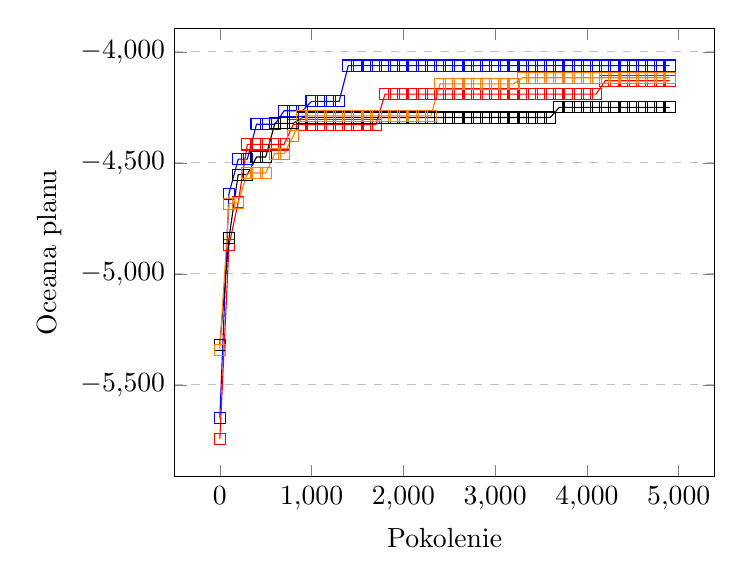
\begin{tikzpicture}
\begin{axis}[
    xlabel={Pokolenie},
    ylabel={Oceana planu},
    ymajorgrids=true,
    grid style=dashed,
]

\addplot[
    color=blue,
    mark=square,
    ]
    coordinates {
(0, -5649.799999999999)(100, -4638.799999999999)(200, -4483.5999999999985)(300, -4483.5999999999985)(400, -4326.4)(500, -4326.4)(600, -4326.4)(700, -4265.599999999999)(800, -4265.599999999999)(900, -4265.599999999999)(1000, -4222.999999999999)(1100, -4222.999999999999)(1200, -4222.999999999999)(1300, -4222.999999999999)(1400, -4061.9999999999995)(1500, -4061.9999999999995)(1600, -4061.9999999999995)(1700, -4061.9999999999995)(1800, -4061.9999999999995)(1900, -4061.9999999999995)(2000, -4061.9999999999995)(2100, -4061.9999999999995)(2200, -4061.9999999999995)(2300, -4061.9999999999995)(2400, -4061.9999999999995)(2500, -4061.9999999999995)(2600, -4061.9999999999995)(2700, -4061.9999999999995)(2800, -4061.9999999999995)(2900, -4061.9999999999995)(3000, -4061.9999999999995)(3100, -4061.9999999999995)(3200, -4061.9999999999995)(3300, -4061.9999999999995)(3400, -4061.9999999999995)(3500, -4061.9999999999995)(3600, -4061.9999999999995)(3700, -4061.9999999999995)(3800, -4061.9999999999995)(3900, -4061.9999999999995)(4000, -4061.9999999999995)(4100, -4061.9999999999995)(4200, -4061.9999999999995)(4300, -4061.9999999999995)(4400, -4061.9999999999995)(4500, -4061.9999999999995)(4600, -4061.9999999999995)(4700, -4061.9999999999995)(4800, -4061.9999999999995)(4900, -4061.9999999999995)
    };
    
\addplot[
    color=red,
    mark=square,
    ]
    coordinates {
(0, -5745.000000000001)(100, -4872.0)(200, -4678.8)(300, -4417.399999999999)(400, -4417.399999999999)(500, -4417.399999999999)(600, -4417.399999999999)(700, -4417.399999999999)(800, -4328.2)(900, -4328.2)(1000, -4328.2)(1100, -4328.2)(1200, -4328.2)(1300, -4328.2)(1400, -4328.2)(1500, -4328.2)(1600, -4328.2)(1700, -4328.2)(1800, -4190.399999999998)(1900, -4190.399999999998)(2000, -4190.399999999998)(2100, -4190.399999999998)(2200, -4190.399999999998)(2300, -4190.399999999998)(2400, -4190.399999999998)(2500, -4190.399999999998)(2600, -4190.399999999998)(2700, -4190.399999999998)(2800, -4190.399999999998)(2900, -4190.399999999998)(3000, -4190.399999999998)(3100, -4190.399999999998)(3200, -4190.399999999998)(3300, -4190.399999999998)(3400, -4190.399999999998)(3500, -4190.399999999998)(3600, -4190.399999999998)(3700, -4190.399999999998)(3800, -4190.399999999998)(3900, -4190.399999999998)(4000, -4190.399999999998)(4100, -4190.399999999998)(4200, -4130.4)(4300, -4130.4)(4400, -4130.4)(4500, -4130.4)(4600, -4130.4)(4700, -4130.4)(4800, -4130.4)(4900, -4130.4)
    };
    
\addplot[
    color=black,
    mark=square,
    ]
    coordinates {
(0, -5320.5999999999985)(100, -4839.4)(200, -4553.4)(300, -4553.4)(400, -4473.999999999999)(500, -4473.999999999999)(600, -4322.4)(700, -4322.4)(800, -4322.4)(900, -4295.999999999999)(1000, -4295.999999999999)(1100, -4295.999999999999)(1200, -4295.999999999999)(1300, -4295.999999999999)(1400, -4295.999999999999)(1500, -4295.999999999999)(1600, -4295.999999999999)(1700, -4295.999999999999)(1800, -4295.999999999999)(1900, -4295.999999999999)(2000, -4295.999999999999)(2100, -4295.999999999999)(2200, -4295.999999999999)(2300, -4295.999999999999)(2400, -4295.999999999999)(2500, -4295.999999999999)(2600, -4295.999999999999)(2700, -4295.999999999999)(2800, -4295.999999999999)(2900, -4295.999999999999)(3000, -4295.999999999999)(3100, -4295.999999999999)(3200, -4295.999999999999)(3300, -4295.999999999999)(3400, -4295.999999999999)(3500, -4295.999999999999)(3600, -4295.999999999999)(3700, -4249.999999999999)(3800, -4249.999999999999)(3900, -4249.999999999999)(4000, -4249.999999999999)(4100, -4249.999999999999)(4200, -4249.999999999999)(4300, -4249.999999999999)(4400, -4249.999999999999)(4500, -4249.999999999999)(4600, -4249.999999999999)(4700, -4249.999999999999)(4800, -4249.999999999999)(4900, -4249.999999999999)
    };
    
\addplot[
    color=orange,
    mark=square,
    ]
    coordinates {
(0, -5342.200000000001)(100, -4684.400000000001)(200, -4679.999999999999)(300, -4545.799999999999)(400, -4545.799999999999)(500, -4545.799999999999)(600, -4458.799999999999)(700, -4458.799999999999)(800, -4379.800000000001)(900, -4288.800000000001)(1000, -4288.800000000001)(1100, -4288.800000000001)(1200, -4288.800000000001)(1300, -4288.800000000001)(1400, -4288.800000000001)(1500, -4288.800000000001)(1600, -4288.800000000001)(1700, -4288.800000000001)(1800, -4288.800000000001)(1900, -4288.800000000001)(2000, -4288.800000000001)(2100, -4288.800000000001)(2200, -4288.800000000001)(2300, -4288.800000000001)(2400, -4144.4)(2500, -4144.4)(2600, -4144.4)(2700, -4144.4)(2800, -4144.4)(2900, -4144.4)(3000, -4144.4)(3100, -4144.4)(3200, -4144.4)(3300, -4116.999999999999)(3400, -4116.999999999999)(3500, -4116.999999999999)(3600, -4116.999999999999)(3700, -4116.999999999999)(3800, -4116.999999999999)(3900, -4116.999999999999)(4000, -4116.999999999999)(4100, -4116.999999999999)(4200, -4116.999999999999)(4300, -4116.999999999999)(4400, -4116.999999999999)(4500, -4116.999999999999)(4600, -4116.999999999999)(4700, -4116.999999999999)(4800, -4116.999999999999)(4900, -4116.999999999999)
    };

\end{axis}
\end{tikzpicture}
\caption{Zmiana oceny planu podczas ewolucji badana co 100 pokoleń. \newline
Rozmiar populacji = 10, Liczba pokoleń = 5000, Liczba mutacji = 3\% krotek \newline
(więcej=lepiej)}\label{rys:graph_3}
\end{figure}

\begin{figure}[H]
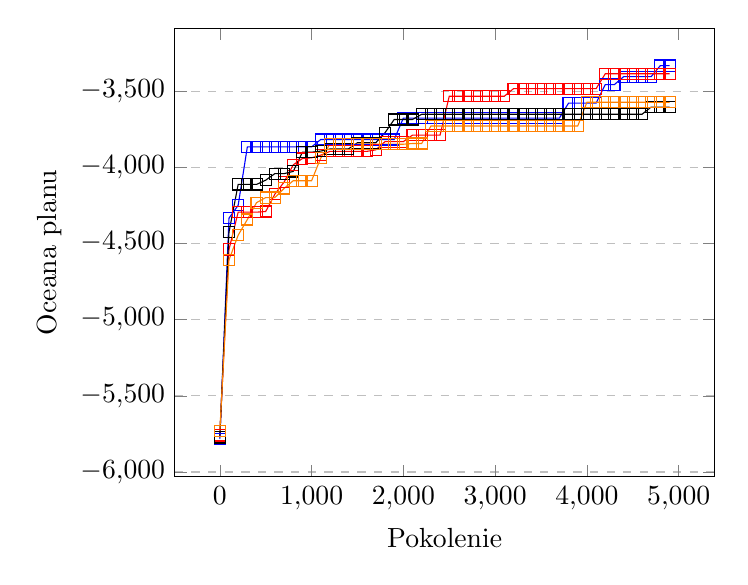
\begin{tikzpicture}
\begin{axis}[
    xlabel={Pokolenie},
    ylabel={Oceana planu},
    ymajorgrids=true,
    grid style=dashed,
]

\addplot[
    color=blue,
    mark=square,
    ]
    coordinates {
(0, -5784.4000000000015)(100, -4332.800000000001)(200, -4248.2)(300, -3864.7999999999997)(400, -3864.7999999999997)(500, -3864.7999999999997)(600, -3864.7999999999997)(700, -3864.7999999999997)(800, -3864.7999999999997)(900, -3864.7999999999997)(1000, -3864.7999999999997)(1100, -3816.0)(1200, -3816.0)(1300, -3816.0)(1400, -3816.0)(1500, -3816.0)(1600, -3816.0)(1700, -3816.0)(1800, -3816.0)(1900, -3816.0)(2000, -3675.5999999999995)(2100, -3675.5999999999995)(2200, -3675.5999999999995)(2300, -3675.5999999999995)(2400, -3675.5999999999995)(2500, -3675.5999999999995)(2600, -3675.5999999999995)(2700, -3675.5999999999995)(2800, -3675.5999999999995)(2900, -3675.5999999999995)(3000, -3675.5999999999995)(3100, -3675.5999999999995)(3200, -3675.5999999999995)(3300, -3675.5999999999995)(3400, -3675.5999999999995)(3500, -3675.5999999999995)(3600, -3675.5999999999995)(3700, -3675.5999999999995)(3800, -3576.999999999999)(3900, -3576.999999999999)(4000, -3576.999999999999)(4100, -3576.999999999999)(4200, -3455.1999999999994)(4300, -3455.1999999999994)(4400, -3403.4)(4500, -3403.4)(4600, -3403.4)(4700, -3403.4)(4800, -3330.599999999999)(4900, -3330.599999999999)
    };
    
    \addplot[
    color=red,
    mark=square,
    ]
    coordinates {
(0, -5759.8)(100, -4538.200000000001)(200, -4293.4)(300, -4293.4)(400, -4293.4)(500, -4289.0)(600, -4175.000000000001)(700, -4096.0)(800, -3982.4000000000005)(900, -3941.0000000000005)(1000, -3936.2000000000003)(1100, -3919.000000000001)(1200, -3894.2000000000003)(1300, -3894.2000000000003)(1400, -3894.2000000000003)(1500, -3894.2000000000003)(1600, -3894.2000000000003)(1700, -3884.2000000000003)(1800, -3830.0000000000005)(1900, -3830.0000000000005)(2000, -3830.0000000000005)(2100, -3787.0)(2200, -3787.0)(2300, -3787.0)(2400, -3787.0)(2500, -3531.7999999999997)(2600, -3531.7999999999997)(2700, -3531.7999999999997)(2800, -3531.7999999999997)(2900, -3531.7999999999997)(3000, -3531.7999999999997)(3100, -3531.7999999999997)(3200, -3482.2)(3300, -3482.2)(3400, -3482.2)(3500, -3482.2)(3600, -3482.2)(3700, -3482.2)(3800, -3482.2)(3900, -3482.2)(4000, -3482.2)(4100, -3482.2)(4200, -3384.3999999999996)(4300, -3384.3999999999996)(4400, -3384.3999999999996)(4500, -3384.3999999999996)(4600, -3384.3999999999996)(4700, -3384.3999999999996)(4800, -3384.3999999999996)(4900, -3384.3999999999996)
    };
    
        \addplot[
    color=black,
    mark=square,
    ]
    coordinates {
(0, -5772.799999999999)(100, -4424.8)(200, -4111.2)(300, -4111.2)(400, -4111.2)(500, -4083.2)(600, -4040.2000000000003)(700, -4040.2000000000003)(800, -4025.8)(900, -3899.600000000001)(1000, -3899.600000000001)(1100, -3892.2)(1200, -3878.6)(1300, -3878.6)(1400, -3878.6)(1500, -3837.1999999999994)(1600, -3837.1999999999994)(1700, -3837.1999999999994)(1800, -3771.7999999999997)(1900, -3684.6)(2000, -3684.6)(2100, -3684.6)(2200, -3650.3999999999996)(2300, -3650.3999999999996)(2400, -3650.3999999999996)(2500, -3650.3999999999996)(2600, -3650.3999999999996)(2700, -3650.3999999999996)(2800, -3650.3999999999996)(2900, -3650.3999999999996)(3000, -3650.3999999999996)(3100, -3650.3999999999996)(3200, -3650.3999999999996)(3300, -3650.3999999999996)(3400, -3650.3999999999996)(3500, -3650.3999999999996)(3600, -3650.3999999999996)(3700, -3650.3999999999996)(3800, -3650.3999999999996)(3900, -3650.3999999999996)(4000, -3650.3999999999996)(4100, -3650.3999999999996)(4200, -3650.3999999999996)(4300, -3650.3999999999996)(4400, -3650.3999999999996)(4500, -3650.3999999999996)(4600, -3650.3999999999996)(4700, -3602.9999999999995)(4800, -3602.9999999999995)(4900, -3602.9999999999995)
    };
    
            \addplot[
    color=orange,
    mark=square,
    ]
    coordinates {
(0, -5731.999999999999)(100, -4607.399999999999)(200, -4444.6)(300, -4341.6)(400, -4231.0)(500, -4197.6)(600, -4197.6)(700, -4137.599999999999)(800, -4086.7999999999993)(900, -4086.7999999999993)(1000, -4086.7999999999993)(1100, -3937.7999999999997)(1200, -3846.9999999999995)(1300, -3846.9999999999995)(1400, -3846.9999999999995)(1500, -3846.9999999999995)(1600, -3846.9999999999995)(1700, -3846.9999999999995)(1800, -3846.9999999999995)(1900, -3846.9999999999995)(2000, -3846.9999999999995)(2100, -3842.3999999999996)(2200, -3842.3999999999996)(2300, -3727.599999999999)(2400, -3727.599999999999)(2500, -3727.599999999999)(2600, -3727.599999999999)(2700, -3727.599999999999)(2800, -3727.599999999999)(2900, -3727.599999999999)(3000, -3727.599999999999)(3100, -3727.599999999999)(3200, -3727.599999999999)(3300, -3727.599999999999)(3400, -3727.599999999999)(3500, -3727.599999999999)(3600, -3727.599999999999)(3700, -3727.599999999999)(3800, -3727.599999999999)(3900, -3727.599999999999)(4000, -3571.1999999999994)(4100, -3571.1999999999994)(4200, -3571.1999999999994)(4300, -3571.1999999999994)(4400, -3571.1999999999994)(4500, -3571.1999999999994)(4600, -3571.1999999999994)(4700, -3571.1999999999994)(4800, -3571.1999999999994)(4900, -3571.1999999999994)
    };

\end{axis}
\end{tikzpicture}
\caption{Zmiana oceny planu podczas ewolucji badana co 100 pokoleń. \newline
Rozmiar populacji = 10, Liczba pokoleń = 5000, Liczba mutacji = 2\% krotek \newline
(więcej=lepiej)}\label{rys:graph_2}
\end{figure}

\begin{figure}[H]
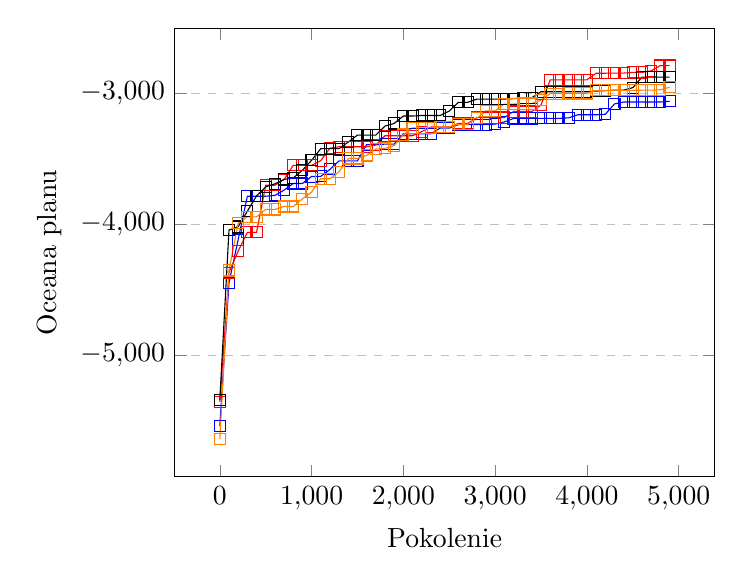
\begin{tikzpicture}
\begin{axis}[
    xlabel={Pokolenie},
    ylabel={Oceana planu},
    ymajorgrids=true,
    grid style=dashed,
]

\addplot[
    color=blue,
    mark=square,
    ]
    coordinates {
(0, -5540.8)(100, -4448.199999999999)(200, -4117.199999999999)(300, -3786.199999999999)(400, -3786.199999999999)(500, -3786.199999999999)(600, -3780.199999999999)(700, -3739.599999999999)(800, -3689.199999999999)(900, -3689.199999999999)(1000, -3635.999999999999)(1100, -3634.3999999999996)(1200, -3581.399999999999)(1300, -3515.999999999999)(1400, -3515.999999999999)(1500, -3515.999999999999)(1600, -3392.1999999999994)(1700, -3392.1999999999994)(1800, -3388.7999999999993)(1900, -3388.7999999999993)(2000, -3309.5999999999995)(2100, -3309.5999999999995)(2200, -3309.5999999999995)(2300, -3309.5999999999995)(2400, -3266.999999999999)(2500, -3266.999999999999)(2600, -3239.999999999999)(2700, -3239.999999999999)(2800, -3239.999999999999)(2900, -3239.999999999999)(3000, -3235.599999999999)(3100, -3219.5999999999995)(3200, -3192.5999999999995)(3300, -3192.5999999999995)(3400, -3192.5999999999995)(3500, -3191.999999999999)(3600, -3191.999999999999)(3700, -3191.999999999999)(3800, -3187.999999999999)(3900, -3164.7999999999997)(4000, -3164.7999999999997)(4100, -3164.7999999999997)(4200, -3160.7999999999997)(4300, -3082.0)(4400, -3067.4)(4500, -3067.4)(4600, -3067.4)(4700, -3067.4)(4800, -3067.4)(4900, -3061.2)
    };
    
\addplot[
    color=red,
    mark=square,
    ]
    coordinates {
(0, -5358.2)(100, -4369.4)(200, -4205.199999999999)(300, -4062.4)(400, -4062.4)(500, -3702.7999999999997)(600, -3702.7999999999997)(700, -3658.7999999999997)(800, -3550.4)(900, -3550.4)(1000, -3550.4)(1100, -3515.1999999999994)(1200, -3419.1999999999994)(1300, -3408.3999999999996)(1400, -3408.3999999999996)(1500, -3408.3999999999996)(1600, -3408.3999999999996)(1700, -3395.799999999999)(1800, -3324.3999999999996)(1900, -3324.3999999999996)(2000, -3324.3999999999996)(2100, -3324.3999999999996)(2200, -3293.3999999999996)(2300, -3257.7999999999993)(2400, -3257.7999999999993)(2500, -3257.7999999999993)(2600, -3230.9999999999995)(2700, -3230.9999999999995)(2800, -3185.9999999999995)(2900, -3185.9999999999995)(3000, -3185.9999999999995)(3100, -3185.9999999999995)(3200, -3139.7999999999997)(3300, -3139.7999999999997)(3400, -3139.7999999999997)(3500, -3090.0)(3600, -2898.0000000000005)(3700, -2898.0000000000005)(3800, -2898.0000000000005)(3900, -2898.0000000000005)(4000, -2898.0000000000005)(4100, -2847.4)(4200, -2847.4)(4300, -2846.4)(4400, -2846.4)(4500, -2841.4)(4600, -2841.4)(4700, -2828.7999999999997)(4800, -2789.2000000000003)(4900, -2789.2000000000003)
    };
    
\addplot[
    color=black,
    mark=square,
    ]
    coordinates {
(0, -5341.799999999998)(100, -4044.9999999999995)(200, -4017.999999999999)(300, -3901.0)(400, -3783.7999999999993)(500, -3715.1999999999994)(600, -3691.7999999999997)(700, -3657.999999999999)(800, -3646.5999999999995)(900, -3588.199999999999)(1000, -3512.1999999999994)(1100, -3423.1999999999994)(1200, -3423.1999999999994)(1300, -3423.1999999999994)(1400, -3372.7999999999997)(1500, -3319.5999999999995)(1600, -3319.5999999999995)(1700, -3319.5999999999995)(1800, -3250.5999999999995)(1900, -3230.5999999999995)(2000, -3173.9999999999995)(2100, -3173.9999999999995)(2200, -3170.0)(2300, -3170.0)(2400, -3170.0)(2500, -3136.2)(2600, -3069.6)(2700, -3069.6)(2800, -3045.6)(2900, -3045.6)(3000, -3045.6)(3100, -3044.4)(3200, -3041.5999999999995)(3300, -3033.9999999999995)(3400, -3033.9999999999995)(3500, -2988.9999999999995)(3600, -2988.9999999999995)(3700, -2988.9999999999995)(3800, -2988.9999999999995)(3900, -2988.9999999999995)(4000, -2988.9999999999995)(4100, -2983.6)(4200, -2980.6)(4300, -2976.6)(4400, -2976.6)(4500, -2957.6)(4600, -2876.7999999999997)(4700, -2876.7999999999997)(4800, -2876.7999999999997)(4900, -2876.7999999999997)
    };
    
\addplot[
    color=orange,
    mark=square,
    ]
    coordinates {
(0, -5640.599999999999)(100, -4352.799999999999)(200, -3992.799999999999)(300, -3943.799999999999)(400, -3943.799999999999)(500, -3886.9999999999986)(600, -3886.9999999999986)(700, -3864.5999999999995)(800, -3864.5999999999995)(900, -3806.399999999999)(1000, -3754.799999999999)(1100, -3652.7999999999997)(1200, -3652.7999999999997)(1300, -3599.0)(1400, -3498.2)(1500, -3498.2)(1600, -3475.2)(1700, -3425.7999999999997)(1800, -3420.9999999999995)(1900, -3399.9999999999995)(2000, -3315.7999999999997)(2100, -3264.7999999999997)(2200, -3264.7999999999997)(2300, -3264.7999999999997)(2400, -3257.7999999999997)(2500, -3257.7999999999997)(2600, -3237.7999999999997)(2700, -3237.7999999999997)(2800, -3191.2)(2900, -3134.9999999999995)(3000, -3134.9999999999995)(3100, -3082.9999999999995)(3200, -3082.9999999999995)(3300, -3079.1999999999994)(3400, -3079.1999999999994)(3500, -3051.1999999999994)(3600, -3002.999999999999)(3700, -3002.999999999999)(3800, -3001.999999999999)(3900, -3001.999999999999)(4000, -3001.999999999999)(4100, -2977.999999999999)(4200, -2977.999999999999)(4300, -2977.999999999999)(4400, -2977.999999999999)(4500, -2977.999999999999)(4600, -2976.9999999999995)(4700, -2976.9999999999995)(4800, -2973.9999999999995)(4900, -2954.5999999999995)
    };

\end{axis}
\end{tikzpicture}
\caption{Zmiana oceny planu podczas ewolucji badana co 100 pokoleń. \newline
Rozmiar populacji = 10, Liczba pokoleń = 5000, Liczba mutacji = 1\% krotek \newline
(więcej=lepiej)}\label{rys:graph_1}
\end{figure}

\begin{figure}[H]
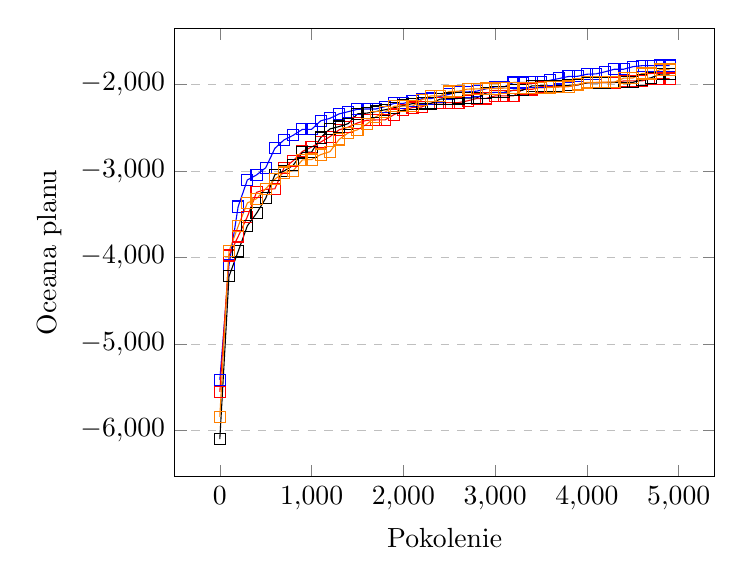
\begin{tikzpicture}
\begin{axis}[
    xlabel={Pokolenie},
    ylabel={Oceana planu},
    ymajorgrids=true,
    grid style=dashed,
]

\addplot[
    color=blue,
    mark=square,
    ]
    coordinates {
(0, -5416.999999999999)(100, -4088.1999999999994)(200, -3408.1999999999994)(300, -3101.1999999999994)(400, -3043.1999999999994)(500, -2960.1999999999994)(600, -2735.2000000000003)(700, -2637.4)(800, -2583.9999999999995)(900, -2515.6)(1000, -2515.6)(1100, -2416.6)(1200, -2388.8)(1300, -2336.8)(1400, -2310.8)(1500, -2283.8)(1600, -2280.2)(1700, -2280.2)(1800, -2253.0)(1900, -2215.0)(2000, -2215.0)(2100, -2191.2)(2200, -2161.8)(2300, -2159.6)(2400, -2134.8)(2500, -2109.8)(2600, -2082.8)(2700, -2082.8)(2800, -2073.8)(2900, -2047.0)(3000, -2024.0)(3100, -2024.0)(3200, -1974.0)(3300, -1974.0)(3400, -1972.0)(3500, -1972.0)(3600, -1948.0)(3700, -1927.0)(3800, -1904.0)(3900, -1902.0)(4000, -1878.2)(4100, -1874.2)(4200, -1849.2)(4300, -1820.2)(4400, -1820.2)(4500, -1791.2000000000003)(4600, -1779.2)(4700, -1779.2)(4800, -1778.2)(4900, -1778.2)
    };
    
    \addplot[
    color=red,
    mark=square,
    ]
    coordinates {
(0, -5553.0)(100, -3974.8)(200, -3754.600000000001)(300, -3526.6000000000004)(400, -3244.2000000000003)(500, -3210.0)(600, -3203.8)(700, -2959.600000000001)(800, -2878.8)(900, -2771.2)(1000, -2720.2000000000003)(1100, -2662.4)(1200, -2600.5999999999995)(1300, -2521.5999999999995)(1400, -2489.6)(1500, -2441.6)(1600, -2410.8)(1700, -2406.8)(1800, -2406.8)(1900, -2344.4)(2000, -2292.4)(2100, -2263.6000000000004)(2200, -2256.6000000000004)(2300, -2212.0)(2400, -2208.8)(2500, -2206.8)(2600, -2206.8)(2700, -2185.8)(2800, -2159.0)(2900, -2158.0)(3000, -2129.0)(3100, -2129.0)(3200, -2129.0)(3300, -2053.8)(3400, -2053.8)(3500, -2022.4)(3600, -2022.4)(3700, -2022.4)(3800, -2021.2)(3900, -2001.4)(4000, -1976.4)(4100, -1974.4)(4200, -1974.4)(4300, -1974.4)(4400, -1955.6000000000001)(4500, -1955.6000000000001)(4600, -1955.6000000000001)(4700, -1928.6000000000001)(4800, -1928.6000000000001)(4900, -1928.6000000000001)
    };
    
        \addplot[
    color=black,
    mark=square,
    ]
    coordinates {
	(0, -6098.999999999999)(100, -4215.799999999999)(200, -3927.7999999999997)(300, -3631.6000000000004)(400, -3487.3999999999996)(500, -3313.4)(600, -3040.6000000000004)(700, -2997.8)(800, -2930.6)(900, -2782.3999999999996)(1000, -2778.3999999999996)(1100, -2610.7999999999997)(1200, -2510.5999999999995)(1300, -2483.5999999999995)(1400, -2449.7999999999997)(1500, -2336.2)(1600, -2328.2)(1700, -2310.0)(1800, -2289.3999999999996)(1900, -2264.3999999999996)(2000, -2239.3999999999996)(2100, -2218.3999999999996)(2200, -2216.3999999999996)(2300, -2216.3999999999996)(2400, -2166.2)(2500, -2159.2)(2600, -2158.2)(2700, -2153.3999999999996)(2800, -2151.3999999999996)(2900, -2095.3999999999996)(3000, -2088.3999999999996)(3100, -2087.2)(3200, -2063.2)(3300, -2063.2)(3400, -2013.3999999999999)(3500, -2010.6)(3600, -2010.6)(3700, -2010.6)(3800, -2006.4)(3900, -2001.1999999999998)(4000, -1978.1999999999998)(4100, -1977.1999999999998)(4200, -1974.8)(4300, -1972.6)(4400, -1972.6)(4500, -1972.6)(4600, -1943.6)(4700, -1918.6)(4800, -1875.6)(4900, -1875.6)
    };
    
            \addplot[
    color=orange,
    mark=square,
    ]
    coordinates {
	(0, -5841.2)(100, -3926.9999999999995)(200, -3636.1999999999994)(300, -3367.6)(400, -3317.6)(500, -3201.6)(600, -3091.7999999999997)(700, -3015.4)(800, -2993.4)(900, -2869.5999999999995)(1000, -2864.5999999999995)(1100, -2807.3999999999996)(1200, -2773.7999999999993)(1300, -2632.399999999999)(1400, -2556.5999999999995)(1500, -2520.7999999999993)(1600, -2456.6000000000004)(1700, -2370.0)(1800, -2316.6000000000004)(1900, -2248.2000000000003)(2000, -2247.2)(2100, -2247.2)(2200, -2173.4000000000005)(2300, -2128.0)(2400, -2128.0)(2500, -2077.8)(2600, -2075.0)(2700, -2050.0)(2800, -2048.0)(2900, -2044.0000000000002)(3000, -2044.0000000000002)(3100, -2039.2000000000003)(3200, -2035.2000000000003)(3300, -2035.2000000000003)(3400, -2035.2000000000003)(3500, -2035.2000000000003)(3600, -2031.0000000000002)(3700, -2025.0000000000002)(3800, -2021.0000000000002)(3900, -1996.0000000000002)(4000, -1973.0000000000002)(4100, -1972.8000000000002)(4200, -1970.8000000000002)(4300, -1968.8)(4400, -1923.8)(4500, -1921.8)(4600, -1869.8)(4700, -1869.8)(4800, -1823.8)(4900, -1823.8)
    };


\end{axis}
\end{tikzpicture}
\caption{Zmiana oceny planu podczas ewolucji badana co 100 pokoleń. \newline
Rozmiar populacji = 10, Liczba pokoleń = 5000, Liczba mutacji = 0.5\% krotek\newline
(więcej=lepiej)}\label{rys:graph_0_5}
\end{figure}

	Ostatni zestaw testów został przeprowadzony po jednym teście z każdego z powyższych zestawów ze zmianą liczby pokoleń na 10000. Takie ustawienie parametrów pozwoliło na znalezienie ciężkich do przejścia progów dla każdego ustawienia. Testy zostały zestawione w ramach jednego wykresu w celu ułatwienia porównania otrzymanych wyników (zob.~rysunek~\ref{rys:graph_all}). Zauważyć można, że dla wartości 3\% oraz 2\% bardzo szybko napotkany zostaje próg nie do przekroczenia przez zbyt dużą losowość. Przez taki próg marnowane są ogromne zasoby obliczeniowe generujące koszty, bez idącego za nimi oczekiwanego wzrostu jakości uzyskanego planu. Z wykresu bardzo szybko wywnioskować można, że najlepszym ustawieniem jest liczba mutacji = 0.5\%. Przez pełen okres wykonywania testu dla tego parametru jakość otrzymywanego planu zwiększała się. Zauważyć można, że optymalnym ustawieniem parametrów dla zaimplementowanego algorytmu jest: rozmiar populacji = 10, liczba pokoleń = 1500, liczba mutacji = 0.5\% liczby krotek w liście (zaokrąglone w dół). Z rysunku przeczytać można, że po przekroczeniu ok.1500 pokolenia dla liczby mutacji = 0.5\% wykres znacznie się spłaszcza co oznacza, że wykorzystując dużą ilość zasobów przez kolejne 8500 pokoleń nie jest otrzymywany już oczekiwany wzrostu jakości.

\begin{figure}[H]
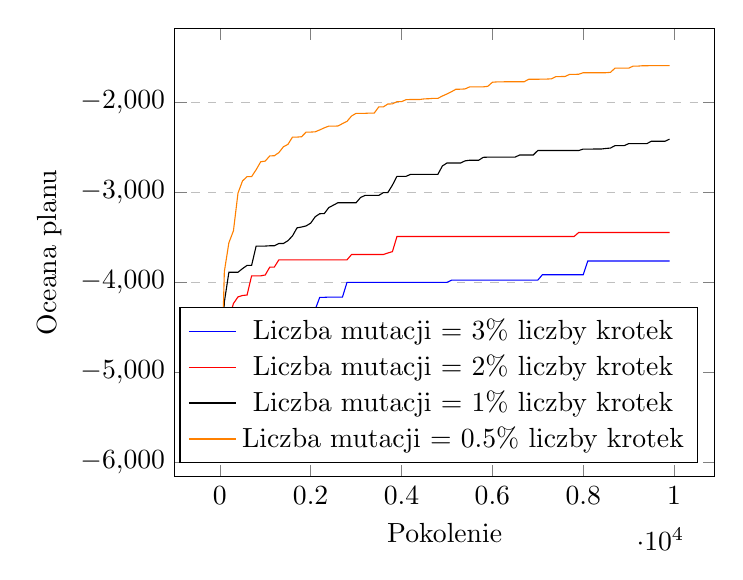
\begin{tikzpicture}
\begin{axis}[
    xlabel={Pokolenie},
    ylabel={Oceana planu},
    ymajorgrids=true,
    grid style=dashed,
    legend pos=south east,
]

\addplot[
    color=blue,
    ]
    coordinates {
	(0, -5694.800000000001)(100, -4786.399999999999)(200, -4730.8)(300, -4730.400000000001)(400, -4701.000000000001)(500, -4524.200000000001)(600, -4524.200000000001)(700, -4354.2)(800, -4354.2)(900, -4354.2)(1000, -4354.2)(1100, -4354.2)(1200, -4354.2)(1300, -4354.2)(1400, -4354.2)(1500, -4354.2)(1600, -4302.000000000001)(1700, -4302.000000000001)(1800, -4302.000000000001)(1900, -4302.000000000001)(2000, -4302.000000000001)(2100, -4302.000000000001)(2200, -4166.4)(2300, -4166.4)(2400, -4163.6)(2500, -4163.6)(2600, -4163.6)(2700, -4163.6)(2800, -3999.9999999999995)(2900, -3999.9999999999995)(3000, -3999.9999999999995)(3100, -3999.9999999999995)(3200, -3999.9999999999995)(3300, -3999.9999999999995)(3400, -3999.9999999999995)(3500, -3999.9999999999995)(3600, -3999.9999999999995)(3700, -3999.9999999999995)(3800, -3999.9999999999995)(3900, -3999.9999999999995)(4000, -3999.9999999999995)(4100, -3999.9999999999995)(4200, -3999.9999999999995)(4300, -3999.9999999999995)(4400, -3999.9999999999995)(4500, -3999.9999999999995)(4600, -3999.9999999999995)(4700, -3999.9999999999995)(4800, -3999.9999999999995)(4900, -3999.9999999999995)(5000, -3999.9999999999995)(5100, -3975.3999999999996)(5200, -3975.3999999999996)(5300, -3975.3999999999996)(5400, -3975.3999999999996)(5500, -3975.3999999999996)(5600, -3975.3999999999996)(5700, -3975.3999999999996)(5800, -3975.3999999999996)(5900, -3975.3999999999996)(6000, -3975.3999999999996)(6100, -3975.3999999999996)(6200, -3975.3999999999996)(6300, -3975.3999999999996)(6400, -3975.3999999999996)(6500, -3975.3999999999996)(6600, -3975.3999999999996)(6700, -3975.3999999999996)(6800, -3975.3999999999996)(6900, -3975.3999999999996)(7000, -3975.3999999999996)(7100, -3915.3999999999996)(7200, -3915.3999999999996)(7300, -3915.3999999999996)(7400, -3915.3999999999996)(7500, -3915.3999999999996)(7600, -3915.3999999999996)(7700, -3915.3999999999996)(7800, -3915.3999999999996)(7900, -3915.3999999999996)(8000, -3915.3999999999996)(8100, -3762.2000000000003)(8200, -3762.2000000000003)(8300, -3762.2000000000003)(8400, -3762.2000000000003)(8500, -3762.2000000000003)(8600, -3762.2000000000003)(8700, -3762.2000000000003)(8800, -3762.2000000000003)(8900, -3762.2000000000003)(9000, -3762.2000000000003)(9100, -3762.2000000000003)(9200, -3762.2000000000003)(9300, -3762.2000000000003)(9400, -3762.2000000000003)(9500, -3762.2000000000003)(9600, -3762.2000000000003)(9700, -3762.2000000000003)(9800, -3762.2000000000003)(9900, -3762.2000000000003)
    };\addlegendentry{Liczba mutacji = 3\% liczby krotek}
    
\addplot[
    color=red,
    ]
    coordinates {
(0, -5366.2)(100, -4468.0)(200, -4408.4)(300, -4235.399999999999)(400, -4161.5999999999985)(500, -4145.999999999998)(600, -4140.5999999999985)(700, -3927.199999999999)(800, -3927.199999999999)(900, -3927.199999999999)(1000, -3917.5999999999995)(1100, -3829.7999999999993)(1200, -3829.7999999999993)(1300, -3748.7999999999993)(1400, -3748.7999999999993)(1500, -3748.7999999999993)(1600, -3748.7999999999993)(1700, -3748.7999999999993)(1800, -3748.7999999999993)(1900, -3748.7999999999993)(2000, -3748.7999999999993)(2100, -3748.7999999999993)(2200, -3748.7999999999993)(2300, -3748.7999999999993)(2400, -3748.7999999999993)(2500, -3748.7999999999993)(2600, -3748.7999999999993)(2700, -3748.7999999999993)(2800, -3748.7999999999993)(2900, -3689.9999999999995)(3000, -3689.9999999999995)(3100, -3689.9999999999995)(3200, -3689.9999999999995)(3300, -3689.9999999999995)(3400, -3689.9999999999995)(3500, -3689.9999999999995)(3600, -3689.9999999999995)(3700, -3672.7999999999993)(3800, -3657.599999999999)(3900, -3489.1999999999994)(4000, -3489.1999999999994)(4100, -3489.1999999999994)(4200, -3489.1999999999994)(4300, -3489.1999999999994)(4400, -3489.1999999999994)(4500, -3489.1999999999994)(4600, -3489.1999999999994)(4700, -3489.1999999999994)(4800, -3489.1999999999994)(4900, -3489.1999999999994)(5000, -3489.1999999999994)(5100, -3489.1999999999994)(5200, -3489.1999999999994)(5300, -3489.1999999999994)(5400, -3489.1999999999994)(5500, -3489.1999999999994)(5600, -3489.1999999999994)(5700, -3489.1999999999994)(5800, -3489.1999999999994)(5900, -3489.1999999999994)(6000, -3489.1999999999994)(6100, -3489.1999999999994)(6200, -3489.1999999999994)(6300, -3489.1999999999994)(6400, -3489.1999999999994)(6500, -3489.1999999999994)(6600, -3489.1999999999994)(6700, -3489.1999999999994)(6800, -3489.1999999999994)(6900, -3489.1999999999994)(7000, -3489.1999999999994)(7100, -3489.1999999999994)(7200, -3489.1999999999994)(7300, -3489.1999999999994)(7400, -3489.1999999999994)(7500, -3489.1999999999994)(7600, -3489.1999999999994)(7700, -3489.1999999999994)(7800, -3489.1999999999994)(7900, -3444.5999999999985)(8000, -3444.5999999999985)(8100, -3444.5999999999985)(8200, -3444.5999999999985)(8300, -3444.5999999999985)(8400, -3444.5999999999985)(8500, -3444.5999999999985)(8600, -3444.5999999999985)(8700, -3444.5999999999985)(8800, -3444.5999999999985)(8900, -3444.5999999999985)(9000, -3444.5999999999985)(9100, -3444.5999999999985)(9200, -3444.5999999999985)(9300, -3444.5999999999985)(9400, -3444.5999999999985)(9500, -3444.5999999999985)(9600, -3444.5999999999985)(9700, -3444.5999999999985)(9800, -3444.5999999999985)(9900, -3444.5999999999985)
    };\addlegendentry{Liczba mutacji = 2\% liczby krotek}
    
\addplot[
    color=black,
    ]
    coordinates {
(0, -5319.400000000001)(100, -4218.4)(200, -3886.9999999999995)(300, -3886.9999999999995)(400, -3886.9999999999995)(500, -3846.399999999999)(600, -3810.999999999999)(700, -3810.999999999999)(800, -3595.6)(900, -3595.6)(1000, -3595.6)(1100, -3592.4)(1200, -3592.4)(1300, -3567.4)(1400, -3567.4)(1500, -3535.7999999999997)(1600, -3482.6)(1700, -3392.8)(1800, -3383.7999999999997)(1900, -3371.4)(2000, -3340.8000000000006)(2100, -3269.600000000001)(2200, -3236.000000000001)(2300, -3233.600000000001)(2400, -3167.2000000000003)(2500, -3140.4)(2600, -3113.4)(2700, -3113.4)(2800, -3113.4)(2900, -3113.4)(3000, -3113.4)(3100, -3054.2000000000003)(3200, -3031.7999999999997)(3300, -3031.7999999999997)(3400, -3031.7999999999997)(3500, -3031.7999999999997)(3600, -3001.0000000000005)(3700, -2999.8)(3800, -2917.4)(3900, -2819.600000000001)(4000, -2819.600000000001)(4100, -2819.600000000001)(4200, -2797.600000000001)(4300, -2797.600000000001)(4400, -2797.600000000001)(4500, -2797.600000000001)(4600, -2797.600000000001)(4700, -2797.600000000001)(4800, -2797.600000000001)(4900, -2704.2000000000007)(5000, -2671.2000000000007)(5100, -2671.2000000000007)(5200, -2671.2000000000007)(5300, -2671.2000000000007)(5400, -2647.2000000000007)(5500, -2640.2000000000003)(5600, -2640.2000000000003)(5700, -2640.2000000000003)(5800, -2608.0000000000005)(5900, -2606.0000000000005)(6000, -2606.0000000000005)(6100, -2606.0000000000005)(6200, -2606.0000000000005)(6300, -2606.0000000000005)(6400, -2606.0000000000005)(6500, -2606.0000000000005)(6600, -2582.0000000000005)(6700, -2582.0000000000005)(6800, -2582.0000000000005)(6900, -2582.0000000000005)(7000, -2532.2)(7100, -2532.2)(7200, -2532.2)(7300, -2532.2)(7400, -2532.2)(7500, -2532.2)(7600, -2532.2)(7700, -2532.2)(7800, -2532.2)(7900, -2532.2)(8000, -2516.0)(8100, -2516.0)(8200, -2516.0)(8300, -2515.2)(8400, -2515.2)(8500, -2509.4)(8600, -2504.6000000000004)(8700, -2478.4)(8800, -2478.4)(8900, -2478.4)(9000, -2455.6000000000004)(9100, -2455.6000000000004)(9200, -2455.6000000000004)(9300, -2455.6000000000004)(9400, -2455.6000000000004)(9500, -2429.2)(9600, -2429.2)(9700, -2429.2)(9800, -2429.2)(9900, -2405.8)
    };\addlegendentry{Liczba mutacji = 1\% liczby krotek}
    
    \addplot[
    color=orange,
    ]
    coordinates {
(0, -5745.199999999999)(100, -3879.0)(200, -3558.4000000000005)(300, -3426.4)(400, -3006.7999999999997)(500, -2870.6)(600, -2822.6)(700, -2822.6)(800, -2746.2000000000003)(900, -2657.8)(1000, -2649.8)(1100, -2592.2000000000003)(1200, -2590.2000000000003)(1300, -2555.6000000000004)(1400, -2490.6000000000004)(1500, -2463.6000000000004)(1600, -2382.8)(1700, -2382.8)(1800, -2378.8)(1900, -2327.0)(2000, -2327.0)(2100, -2323.8)(2200, -2302.8)(2300, -2279.8)(2400, -2260.4)(2500, -2260.4)(2600, -2259.6000000000004)(2700, -2232.8)(2800, -2207.8)(2900, -2148.2)(3000, -2118.2)(3100, -2118.2)(3200, -2118.2)(3300, -2115.4)(3400, -2115.4)(3500, -2046.4000000000003)(3600, -2046.4000000000003)(3700, -2014.4)(3800, -2013.4)(3900, -1988.4)(4000, -1988.4)(4100, -1966.4)(4200, -1964.4)(4300, -1964.4)(4400, -1964.4)(4500, -1957.4)(4600, -1955.6000000000001)(4700, -1951.6000000000001)(4800, -1951.6000000000001)(4900, -1925.6000000000001)(5000, -1902.6000000000001)(5100, -1877.6)(5200, -1849.8)(5300, -1849.6000000000001)(5400, -1846.6000000000001)(5500, -1823.6000000000001)(5600, -1823.6000000000001)(5700, -1823.6000000000001)(5800, -1823.6000000000001)(5900, -1817.6000000000001)(6000, -1772.4)(6100, -1768.4)(6200, -1768.4)(6300, -1766.4)(6400, -1766.4)(6500, -1766.4)(6600, -1766.4)(6700, -1766.4)(6800, -1739.4)(6900, -1739.4)(7000, -1739.0)(7100, -1737.0)(7200, -1737.0)(7300, -1734.0)(7400, -1709.0)(7500, -1709.0)(7600, -1708.0)(7700, -1685.0)(7800, -1685.0)(7900, -1683.0)(8000, -1666.0)(8100, -1666.0)(8200, -1666.0)(8300, -1666.0)(8400, -1666.0)(8500, -1666.0)(8600, -1662.0)(8700, -1615.8)(8800, -1615.8)(8900, -1615.8)(9000, -1615.8)(9100, -1592.8)(9200, -1592.8)(9300, -1588.8)(9400, -1588.8)(9500, -1586.8)(9600, -1586.8)(9700, -1586.8)(9800, -1586.8)(9900, -1586.8)
    };\addlegendentry{Liczba mutacji = 0.5\% liczby krotek}
    


\end{axis}
\end{tikzpicture}
\caption{Zmiana oceny planu podczas ewolucji badana co 100 pokoleń. \newline
Rozmiar populacji = 10, Liczba pokoleń = 5000\newline
(więcej=lepiej)}\label{rys:graph_all}
\end{figure}
	
	 


\chapter{Instrukcja użytkowania}
\section{Strona główna}
Strona główna~(zob.~rysunek~\ref{rys:main}) aplikacji została stworzona na bazie szablonu Bootstrap o nazwie One Page Wonder~\cite{opw}. Zawiera ona krótki opis aplikacji, a także korzyści płynących z wykorzystania jej dla planistów, nauczycieli oraz uczniów. Pasek menu znajdujący się zawsze na górze strony jest stałym elementem aplikacji pojawiającym się w każdym z widoków. Pozwala on na przejście do widoków logowania i rejestracji, a w przypadku gdy użytkownik jest już zalogowany na wylogowanie lub przejście do widoku szkoły. 
\begin{figure}[!ht]
\centering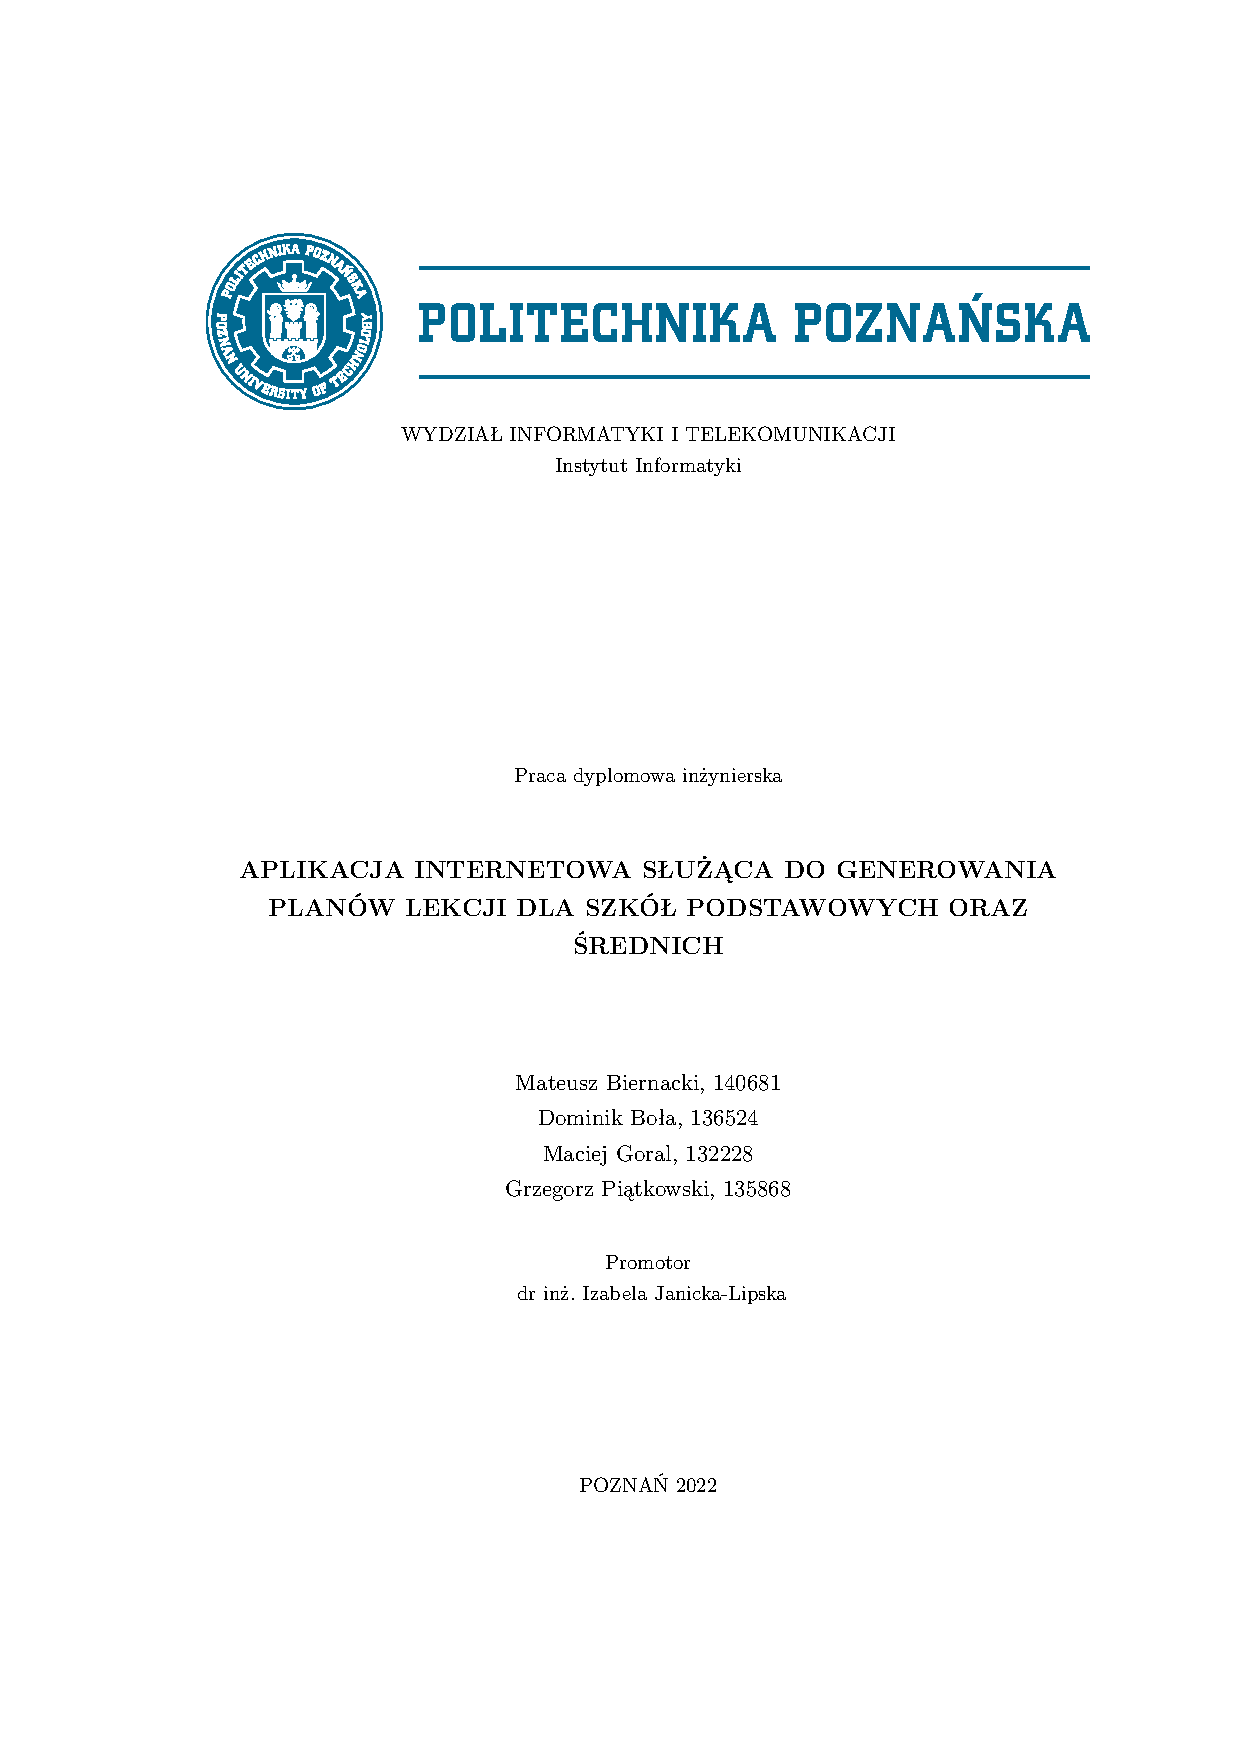
\includegraphics[width=\textwidth]{figures/main}
\caption{Aplikacja internetowa -- Strona główna}\label{rys:main}
\end{figure}
\section{Widok szkoły}
Widok szkoły~(zob.~rysunek~\ref{rys:school}) pozwala na przejście do dodawania danych potrzebnych do wygenerowania planu, a przypadku gdy plan został już wygenerowany jest również miejscem, w którym jest on wyświetlany. Rozkład zajęć jest możliwy do wyświetlenia na trzy sposoby -- z podziałem na klasy, nauczycieli lub sale lekcyjne.

\begin{figure}[!ht]
\centering\includegraphics[width=\textwidth]{figures/school}
\caption{Aplikacja internetowa -- Widok szkoły}\label{rys:school}
\end{figure}
\section{Rejestracja}
Widok rejestracji~(zob.~rysunek~\ref{rys:register}) umożliwia utworzenie konta w serwisie. Od użytkownika wymaga się podania adresu e-mail, nazwy użytkownika oraz hasła. Adres e-mail musi być unikatowy. Wynika to z konieczności weryfikacji konta poprzez wiadomość wysłaną przy pomocy serwera SMTP. Rozwiązanie to ma na celu zapobieganie atakom na stronę poprzez masowe tworzenie nowych kont. 
\begin{figure}[!ht]
\centering\includegraphics[width=\textwidth]{figures/register}
\caption{Aplikacja internetowa -- Widok rejestracji}\label{rys:register}
\end{figure}
\section{Logowanie}
Widok logowania~(zob.~rysunek~\ref{rys:login}) pozwala na dostęp do konta i zapisanych na nim danych z dowolnego urządzenia. Do uwierzytelnienia użytkownika wykorzystywany jest adres e-mail oraz hasło podane w procesie rejestracji. Powodzenie procesu logowania powoduje otrzymanie przez aplikację tokenu JWT, zapisywanego w pamięci przeglądarki. W przypadku utraty hasła użytkownik posiada możliwość odzyskania go po podaniu adresu e-mail powiązanego z istniejącym kontem.
\begin{figure}[h]
\centering\includegraphics[width=\textwidth]{figures/login}
\caption{Aplikacja internetowa -- Widok logowania}\label{rys:login}
\end{figure}
\section{Ankieta}
Widok ankiety~(zob.~rysunek~\ref{rys:poll}) pozwala nauczycielowi na podanie preferencji godzinowych pracy. W przeciwieństwie do pozostałych widoków jest on dostępny jedynie poprzez bezpośredni link wysyłany w wiadomości e-mail. Takie rozwiązanie sprawia, że jedynym użytkownikiem, od którego wymagane jest posiadanie konta jest planista. Nauczyciele jako użytkownicy bez konta są identyfikowani dzięki unikalności adresu URL.
\begin{figure}[!ht]
\centering\includegraphics[width=\textwidth]{figures/poll}
\caption{Aplikacja internetowa -- Widok ankiet dla nauczycieli}\label{rys:poll}
\end{figure}
\section{Dodawanie przedmiotów}
Widok dodawania przedmiotów~(zob.~rysunek~\ref{rys:subject}) stanowi pierwszy krok w procesie podawania danych koniecznych do wygenerowania planu zajęć. 
 
\begin{figure}[h]
\centering\includegraphics[width=\textwidth]{figures/subject}
\caption{Aplikacja internetowa -- Widok dodawania przedmiotów}\label{rys:subject}
\end{figure}
W celu dodawania przedmiotu należy podać jedynie jego nazwę. Powiązania z nauczycielami, salami lekcyjnymi i klasami będą mogły być wprowadzone w kolejnych krokach. Podanie nazw przedmiotów na początku procesu dodawania danych pozwala na to, aby w późniejszych etapach mogły być one wybierane z listy rozwijanej. Zapobiega to konieczności wielokrotnego ręcznego wprowadzania tych samych informacji i ułatwia tworzenie powiązań w bazie danych. W lewej części ekranu znajduje się lista już wprowadzonych przedmiotów. Wybranie z nich jednego powoduje przejście do ekranu edycji. Analogiczne rozwiązanie zostało zastosowane we wszystkich kolejnych ekranach dodawania danych.
\section{Dodawanie nauczycieli}
W widoku dodawania nauczycieli~(zob.~rysunek~\ref{rys:teacher}) planista ma możliwość wprowadzenia danych personelu dydaktycznego oraz jego powiązań z przedmiotami. Każdy nauczyciel musi posiadać imię i nazwisko, unikalny w skali szkoły adres e-mail oraz przynajmniej jeden prowadzony przedmiot. Ekran umożliwia dodanie kolejnych prowadzonych przedmiotów w przypadku, gdy nauczyciel prowadzi więcej niż jeden. Planista ma również możliwość wysłania ankiet dyspozycyjności ma adresy e-mail do tej pory wprowadzonych nauczycieli.
\begin{figure}[!ht]
\centering\includegraphics[width=\textwidth]{figures/teacher}
\caption{Aplikacja internetowa -- Widok dodawania nauczycieli}\label{rys:teacher}
\end{figure}
\section{Dodawanie sal lekcyjnych}
\begin{figure}[h]
\centering\includegraphics[width=\textwidth]{figures/classroom}
\caption{Aplikacja internetowa -- Widok dodawania sali lekcyjnych}\label{rys:classroom}
\end{figure}
Dodanie informacji o salach lekcyjnych~(zob.~rysunek~\ref{rys:classroom}) stanowi trzeci krok dodawania danych. Sala lekcyjna musi posiadać nazwę, a opcjonalnie także listę przedmiotów, które mogą być w  niej prowadzone. W przypadku, gdy nie zostanie wybrany żaden preferowany przedmiot, sala zostaje uznana za salę zwykłą, co oznacza, że będzie mógł być w niej prowadzony dowolny przedmiot.
\section{Dodawanie klas}
Ostatnim etapem w procesie dodawania niezbędnych danych jest wprowadzenie parametrów klas~(zob.~rysunek~\ref{rys:class}). Każda klasa musi posiadać nazwę oraz listę przedmiotów, które mają się pojawić w jej planie zajęć. Każdy element listy musi zawierać nazwę przedmiotu, liczbę godzin lekcyjnych w tygodniu przeznaczonych na przedmiot oraz opcjonalnie prowadzącego przedmiot. Brak wyboru nauczyciela umożliwia przypisanie zajęć dowolnemu prowadzącemu dany przedmiot.
\begin{figure}[!ht]
\centering\includegraphics[width=\textwidth]{figures/class}
\caption{Aplikacja internetowa -- Widok dodawania klas}\label{rys:class}
\end{figure}
\section{Edycja danych}
Dla czterech powyższych ekranów istnieją odpowiadające im ekrany edycji danych.

\begin{figure}[h]
\centering\includegraphics[width=\textwidth]{figures/edit}
\caption{Aplikacja internetowa -- Widok edycji danych nauczyciela}\label{rys:edit}
\end{figure}

Ze względu na ich analogiczną budowę ich struktura zostanie omówiona na bazie widoku edycji danych nauczyciela~(zob.~rysunek~\ref{rys:edit}). Przejście do tego ekranu umożliwiają przyciski znajdujące się po prawej stronie widoku dodawania nauczycieli. Przyciski te są wciąż obecne w widoku edycji i pozwalają na przechodzenie pomiędzy danymi poszczególnych osób bez zapisywania wprowadzonych zmian. W chwili przejścia do ekranu edycji pola z danymi zostają uzupełnione pierwotnie wprowadzonymi informacjami o nauczycielu. Takie rozwiązanie ma celu zapobieganie konieczności ponownego wprowadzania wszystkich danych, w przypadku gdy tylko niektóre z nich wymagają zmian. Przyciski u dołu pozwalają na zapisanie wprowadzonych zmian, powrót do ekranu dodawania nauczycieli lub całkowite usunięcie nauczyciela z bazy danych.


\chapter{Zakończenie}

\section{Podsumowanie pracy}

Celem pracy inżynierskiej była implementacja aplikacji internetowej służącej do generacji planów zajęć dla szkół podstawowych oraz średnich. Motywacją do podjęcia takiego tematu, był fakt, że układanie planów zajęć jest zadaniem trudnym~\cite{trudne_plany_a}~\cite{trudne_plany_b}. W dużych szkołach plan może być układany nawet miesiącami. Zautomatyzowanie procesu układania planu zajęć może zaoszczędzić pracy osobom, które za to odpowiadają. Dodatkowo pojawia się potrzeba dobrego gospodarowania czasem uczniów oraz nauczycieli, czego ręcznie układane plany zajęć nie zapewniają.

Szczególna uwaga została zwrócona na to, by aplikacja wyświetlała swoją zawartość w przeglądarce w sposób czytelny oraz estetyczny. Jest to jedyna część aplikacji, z którą potencjalny klient miałby bezpośrednią styczność. Oznacza to, że wygląd zawartości wpływałby w znacznym stopniu na odbiór aplikacji przez użytkownika.

Niezwykle ważne było założenie, że projekt ma powstawać w metodyce \textit{DevOps}. Czas włożony na wdrożenie praktyk \textit{DevOps} zaowocował dużą oszczędnością czasu. Fakt, że programowane rozwiązania były wdrażane automatycznie na projektowe maszyny, spowodował znaczne przyśpieszenie postępu prac. Pozwoliło to również na ograniczenie zagrożeń związanych z jednoczesną edycją kodu źródłowego przez więcej niż jedną osobę.

Kluczową częścią projektu była implementacja algorytmu układającego plan zajęć. Problem ten był na tyle złożony, że sam wybór sposobu podejścia nie był trywialną częścią. Ostatecznie zdecydowano się na podejście ewolucyjne. Algorytm pozwala na ułożenie dobrych planów zajęć w szybkim czasie (w porównaniu z ręcznym układaniem planów).

Działanie strony serwerowej zostało oparte na darmowej platformie programistycznej \textit{Django}. Wybór ten zapewnił bezpieczne oraz wydajne działanie całej aplikacji. Część serwerowa obsługuje wszystkie żądania klienta, sprawia to, że jej poprawne działanie było ważną częścią projektu.

Wszystkie wymagania wspomniane w podrozdziale 3.4 udało się spełnić.

\section{Możliwości rozwoju aplikacji}

Do aplikacji Autoplaner może zostać w przeszłości dodana funkcjonalność generowania planów zajęć dostosowanych do warunków panujących na uczelniach. Wymagałoby to dodania możliwości swobodnego dzielenia klas na grupy oraz grup na jeszcze mniejsze podgrupy. Przykładowo kierunek studiów można podzielić na cztery grupy dziekańskie, a każdą grupę dziekańską na dwie grupy laboratoryjne. Należałoby również przyjąć sytuację, w której jedna osoba może należeć do kilku grup jednocześnie, gdzie pierwsza grupa może nie być podgrupą drugiej grupy, np. do grupy dziekańskiej i do grupy językowej.

Zaimplementowana może również zostać możliwość określenia rozmiaru grup oraz sal, tzn. liczba osób przynależna do konkretnej grupy oraz liczba miejsc siedzących dostępnych w konkretnej sali. Algorytm musiałby wtedy sprawdzać, czy dana sala ma wystarczającą liczbę miejsc, aby przeprowadzić zajęcia dla konkretnej grupy.

Ciekawym rozwinięciem aplikacji może być również automatyczne tworzenie wirtualnych maszyn, na których działałby wyłącznie algorytm. Każde żądanie utworzenia planu zajęć powodowałoby automatyczne utworzenie maszyny wirtualnej, na której będą wykonywane odpowiednie obliczenia. W przypadku tworzenia kilku planów jednocześnie wyeliminowałoby to problem dzielenia zasobów przez szkoły. W takim modelu za utrzymanie konkretnej maszyny odpowiadałaby szkoła, a po wykonaniu odpowiednich obliczeń maszyna wirtualna zostałaby usunięta. Wymagałoby to głębokiej integracji z konkretnym dostawcą usług internetowych takich jak np. \textit{Amazon Web Services}.

Następną możliwą funkcjonalnością jest pokazywanie czasu potrzebnego do wygenerowania konkretnego planu zajęć oraz określania, czy przy generacji planu bardziej klientowi będzie zależeć na czasie wygenerowania planu, czy na jego dobrej jakości. W połączeniu z funkcjonalnością z poprzedniego akapitu klient mógłby nawet określić parametry generowanej wirtualnej maszyny.

W celu komercjalizacji projektu konieczna byłaby integracja z wybranym operatorem płatności internetowych. Klient mógłby wtedy płacić od razu z poziomu aplikacji. Cena usługi generacji planu zajęć byłaby uzależniona od czasu potrzebnego na wygenerowanie planu zajęć. Należałoby wtedy uwzględnić to, że w przypadku jednoczesnej pracy kilku instancji algorytmu, działanie algorytmu byłoby dłuższe. Wspomniany problem nie występowałby w przypadku zaimplementowania funkcjonalności automatycznej generacji wirtualnych maszyn.

%--------------------------------------
% Literatura
%--------------------------------------

\bibliographystyle{plain}{\raggedright\sloppy\small\bibliography{bibliografia}}

%--------------------------------------
% Informacja o prawach autorskich
%--------------------------------------

\ppcolophon

\end{document}
